\section{Models and Experiments}
To measure the existence of bias in NER systems, we evaluated five named entity models used in research and industry. We used Flair~\cite{akbik2018coling,akbik-etal-2019-flair}, CoreNLP version 3.9~\cite{manning-EtAl:2014:P14-5,Finkel:2005:INI:1219840.1219885}, and Spacy version 2.1 with small, medium, and large models.\footnote{\small{\url{https://spacy.io}}}
We test these models against 139 years of U.S. census data\footnote{\small{\url{http://www.ssa.gov/oact/babynames/names.zip}}} from years 1880 to 2018. Our benchmark evaluates these models based upon how well they recognize these names as a PERSON entity. 
\subsection{Benchmark}
Our benchmark dataset consists of nine templates listed in Table \ref{Templates} which are templated sentences that start with the existing names in the census data followed by a sentence that represents a human-like activity. The aim was to test the performance of the NER from different perspectives. Template 1, containing just the name, purely tests the name itself and reveals something about the distribution of the training data. Template 4 is designed to direct the model to tag the name as a person. Template 3 may reveal more subtle gender bias that stems from society as, historically, men have received greater levels of education from women. It is possible that the error rate may be even higher for female names under Template 3.

%The aim was to make it easier for the model to recognize these names as being a PERSON entity; however, our results show that even with these simple templated sentences, the models still confuse PERSON entities with other entity types, such as LOCATION, ORGANIZATION, or MISCELLANEOUS. We separated this benchmark by the year and gender of the name as provided in the census data.
\begin{figure*}[!bt]
% \includegraphics[width=\textwidth,height=0.9\textwidth,trim=0.5cm 0.2cm 0.4cm 0cm,clip=true]{results1.pdf}
%\begin{subfigure}[b]{\textwidth}
%\centering
% \includegraphics[width=1\textwidth,height=0.16\textwidth,trim=0cm 0cm 0cm 0cm,clip=true]{weighted_combined.pdf}
\begin{subfigure}[b]{0.33\textwidth}
\caption{Error Type-1 Weighted}
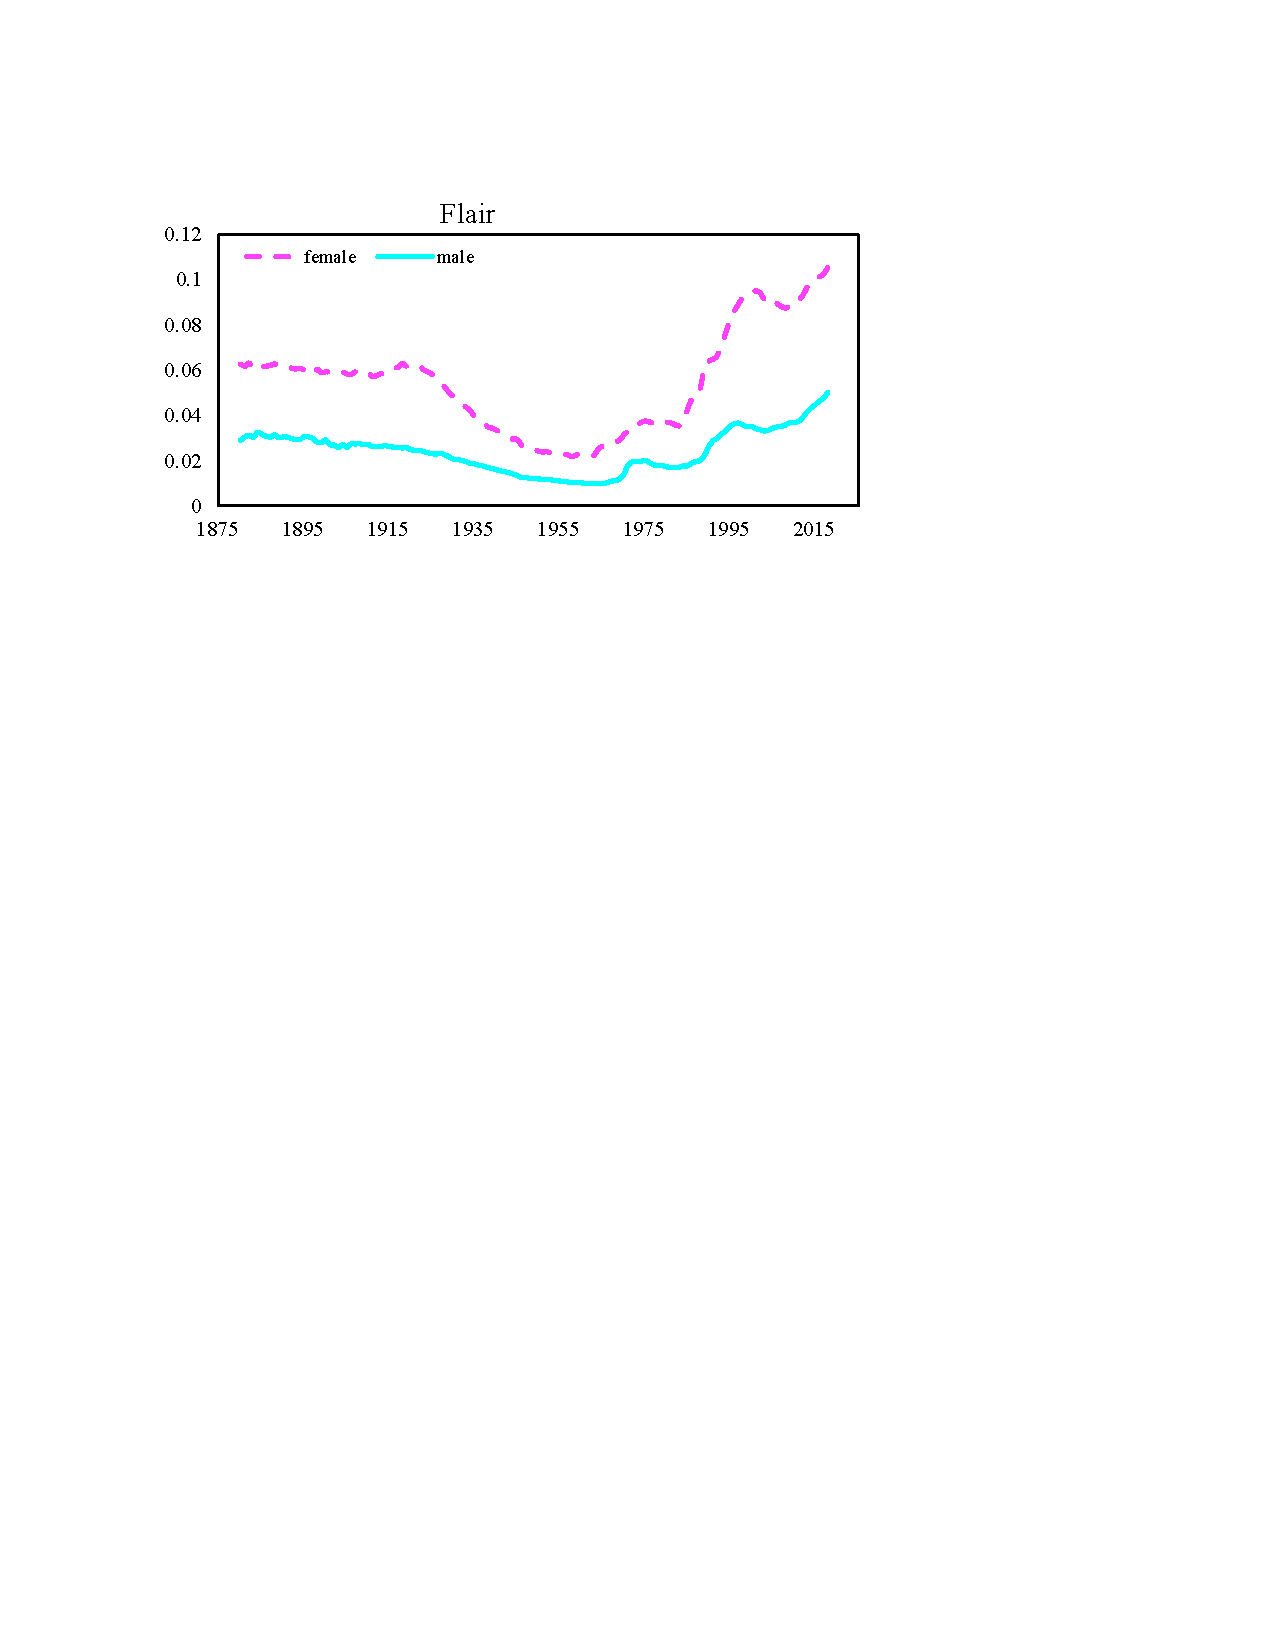
\includegraphics[width=\textwidth,height=0.5\textwidth,trim=0cm 0cm 0cm 0cm,clip=true]{./images/weighted_type1/weighted_type1_1.pdf}
\end{subfigure}
\begin{subfigure}[b]{0.33\textwidth}
\caption{Error Type-2 Weighted}
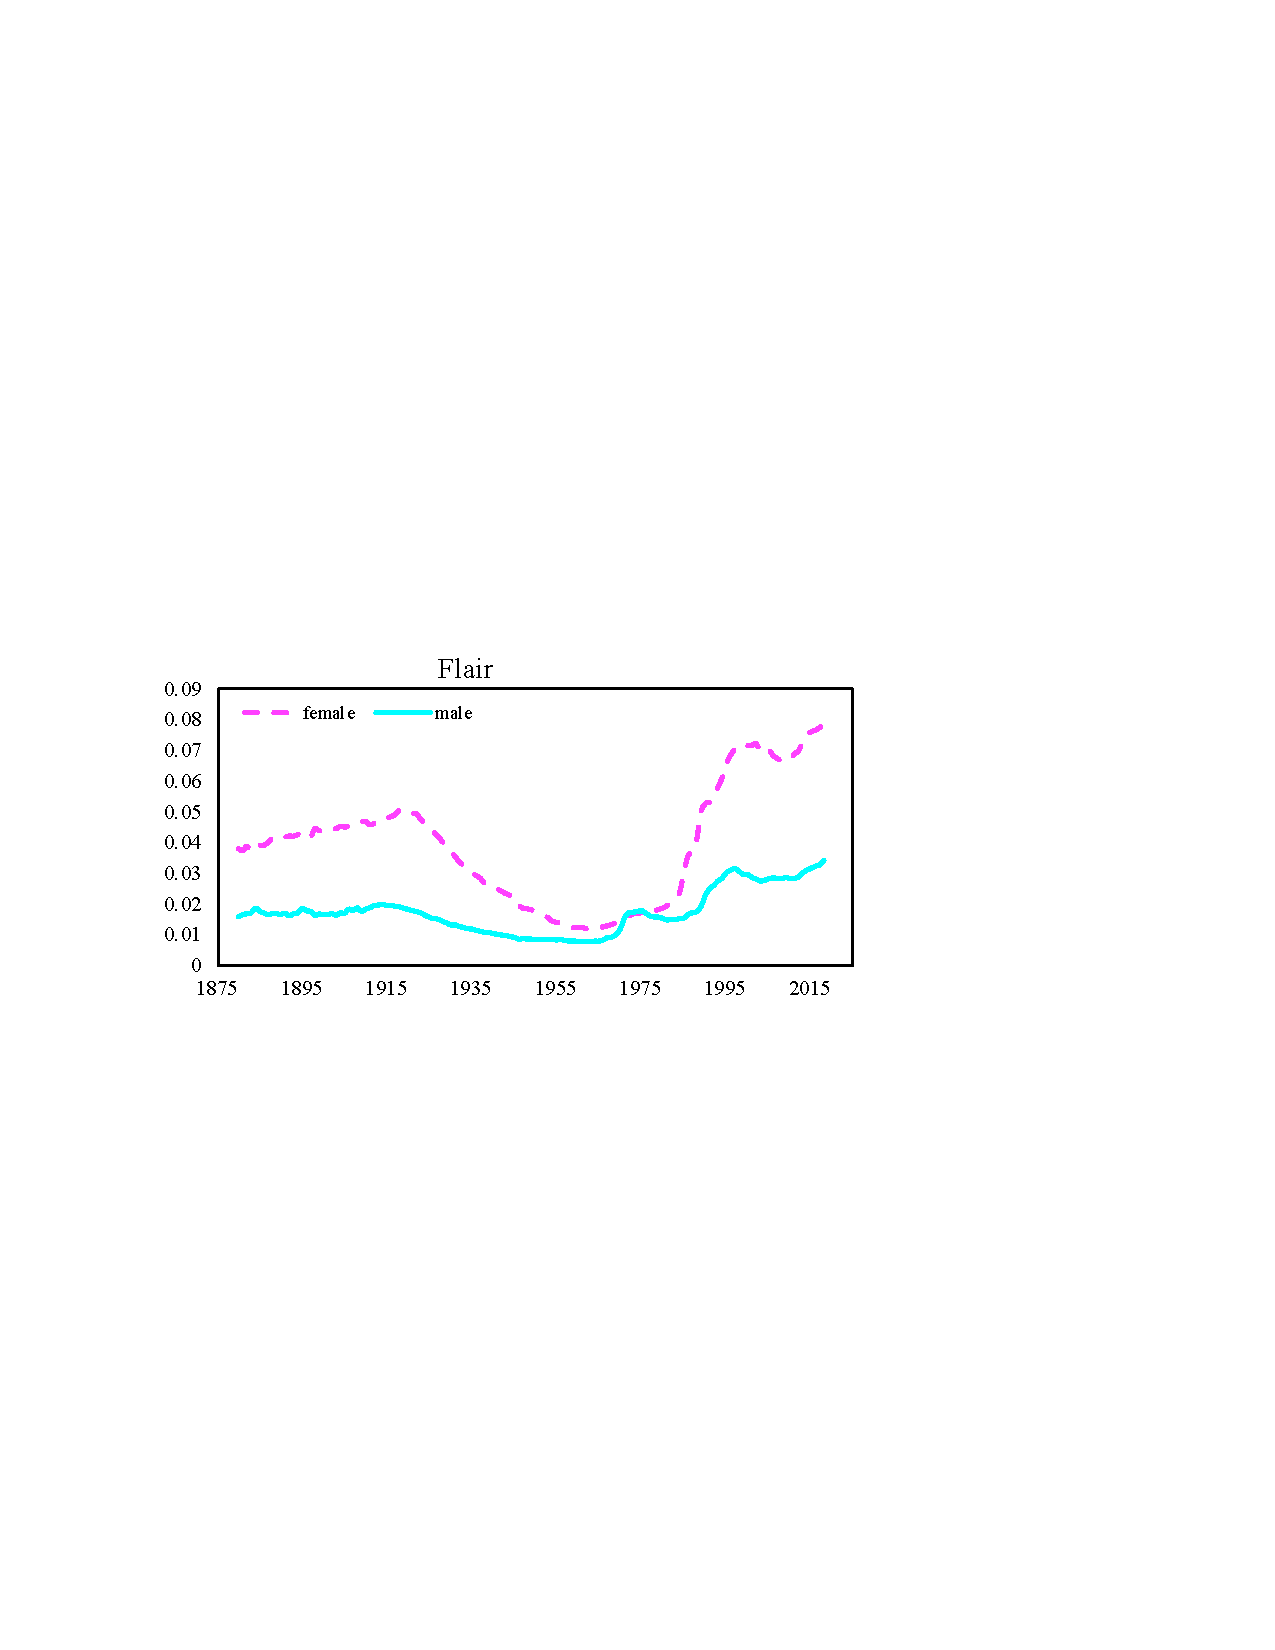
\includegraphics[width=\textwidth,height=0.5\textwidth,trim=0cm 0cm 0cm 0cm,clip=true]{./images/weighted_type2/weighted_type2_1.pdf}
\end{subfigure}
\begin{subfigure}[b]{0.33\textwidth}
\caption{Error Type-3 Weighted}
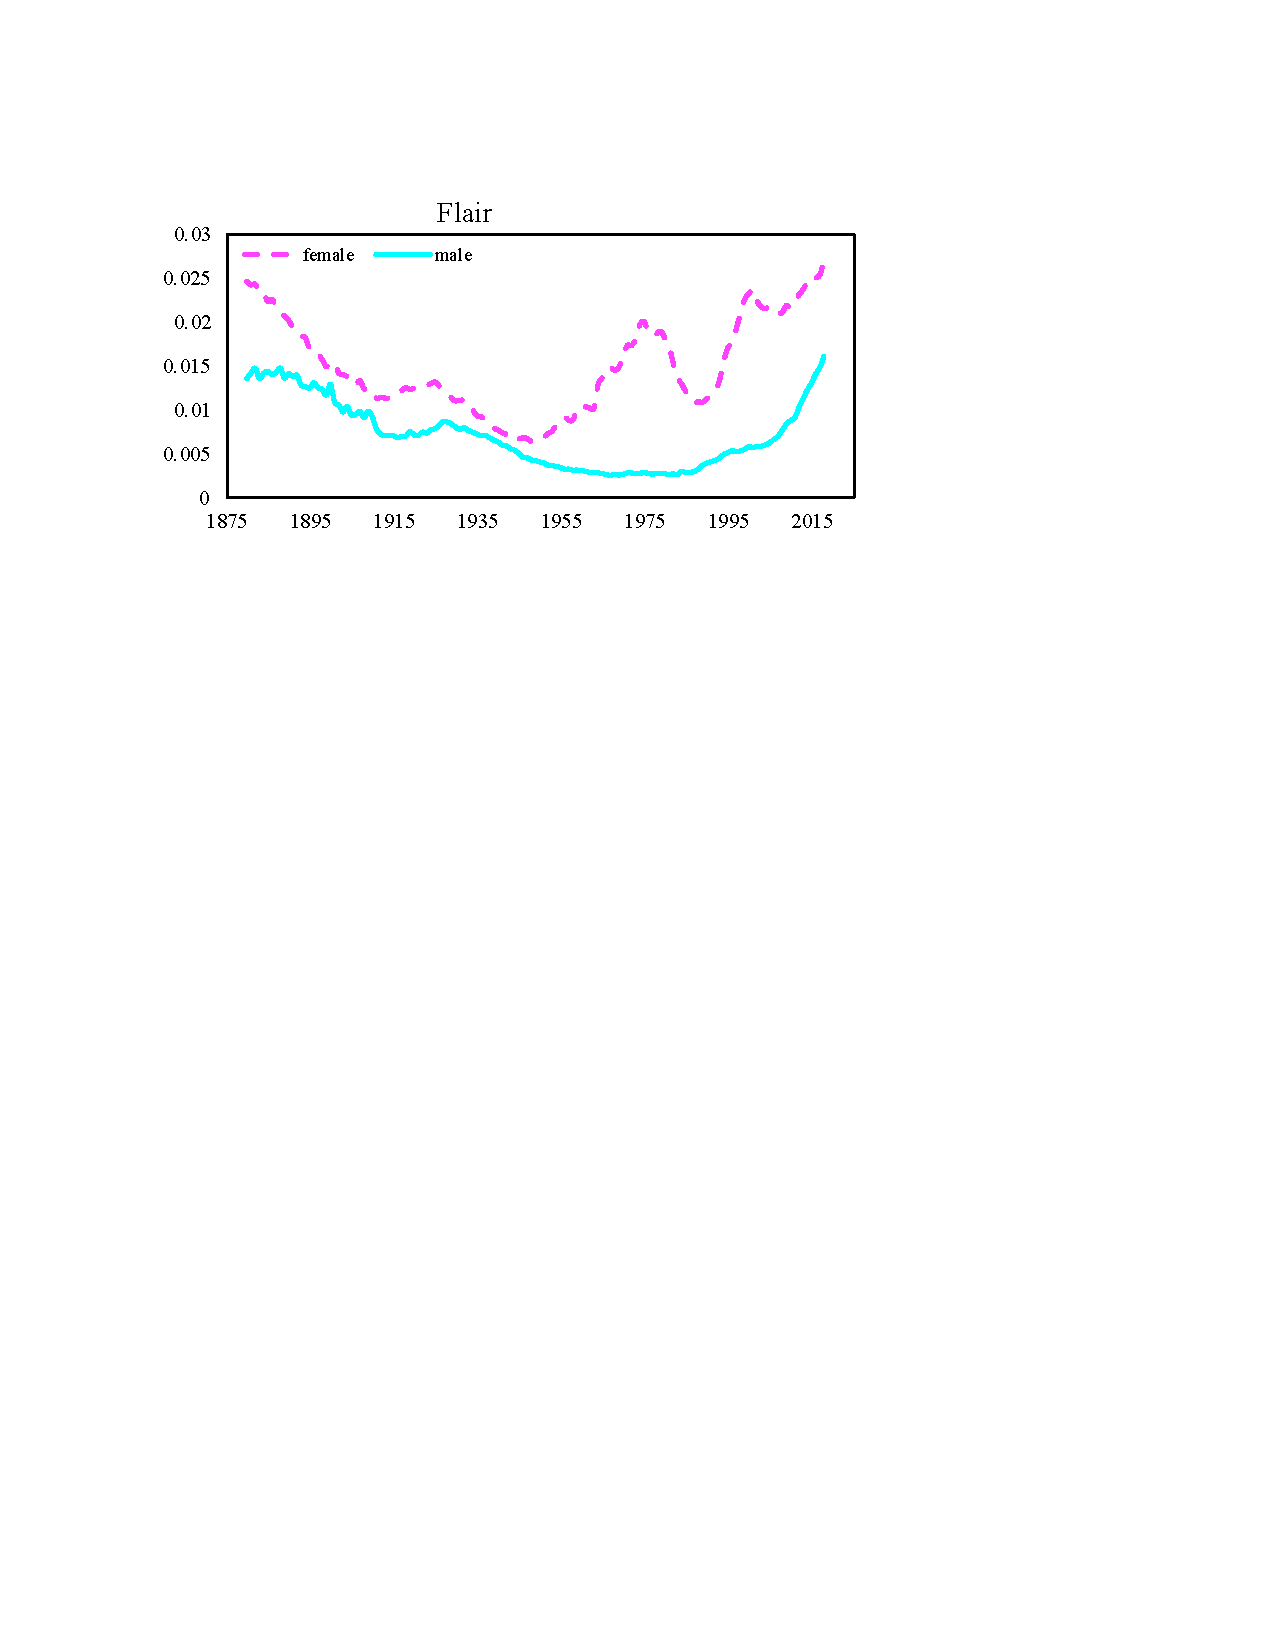
\includegraphics[width=\textwidth,height=0.5\textwidth,trim=0cm 0cm 0cm 0cm,clip=true]{./images/weighted_type3/weighted_type3_1.pdf}
\end{subfigure}
\begin{subfigure}[b]{0.33\textwidth}
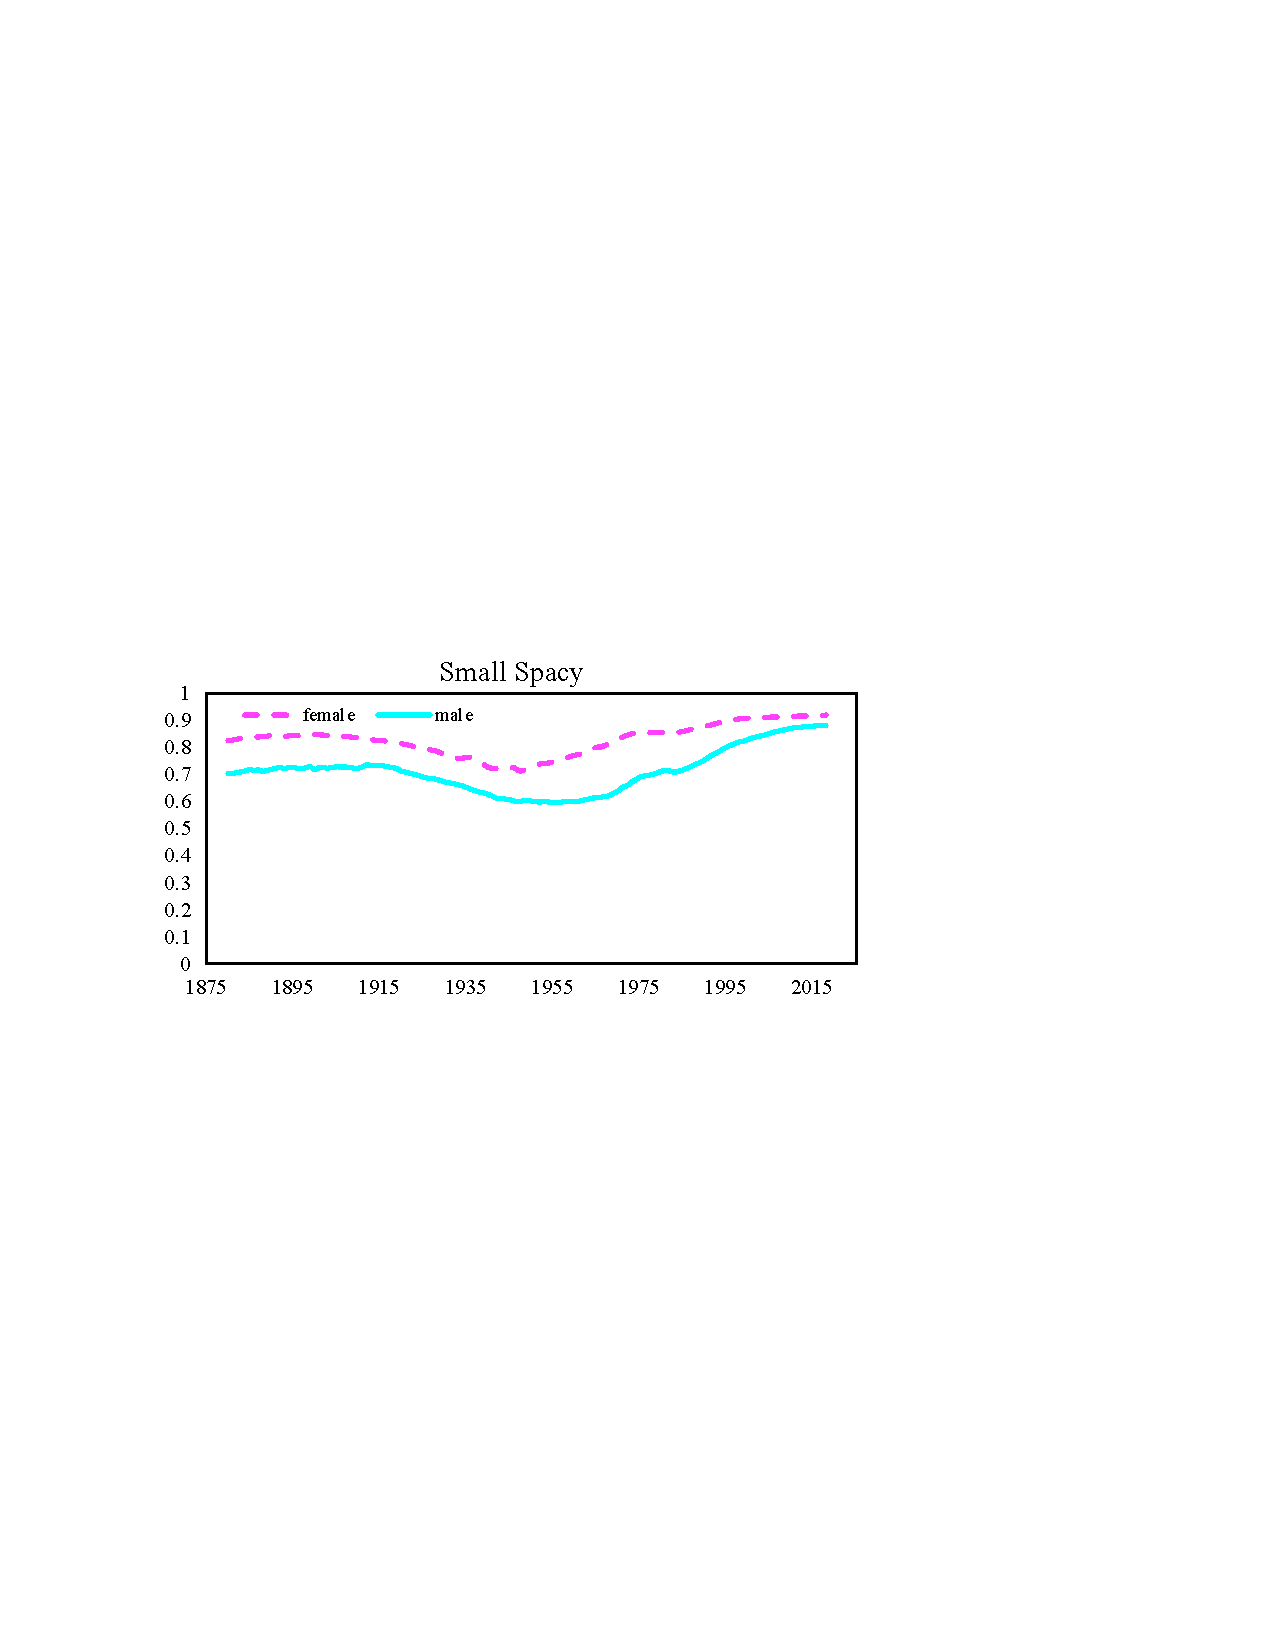
\includegraphics[width=\textwidth,height=0.5\textwidth,trim=0cm 0cm 0cm 0cm,clip=true]{./images/weighted_type1/weighted_type1_2.pdf}
\end{subfigure}
\begin{subfigure}[b]{0.33\textwidth}
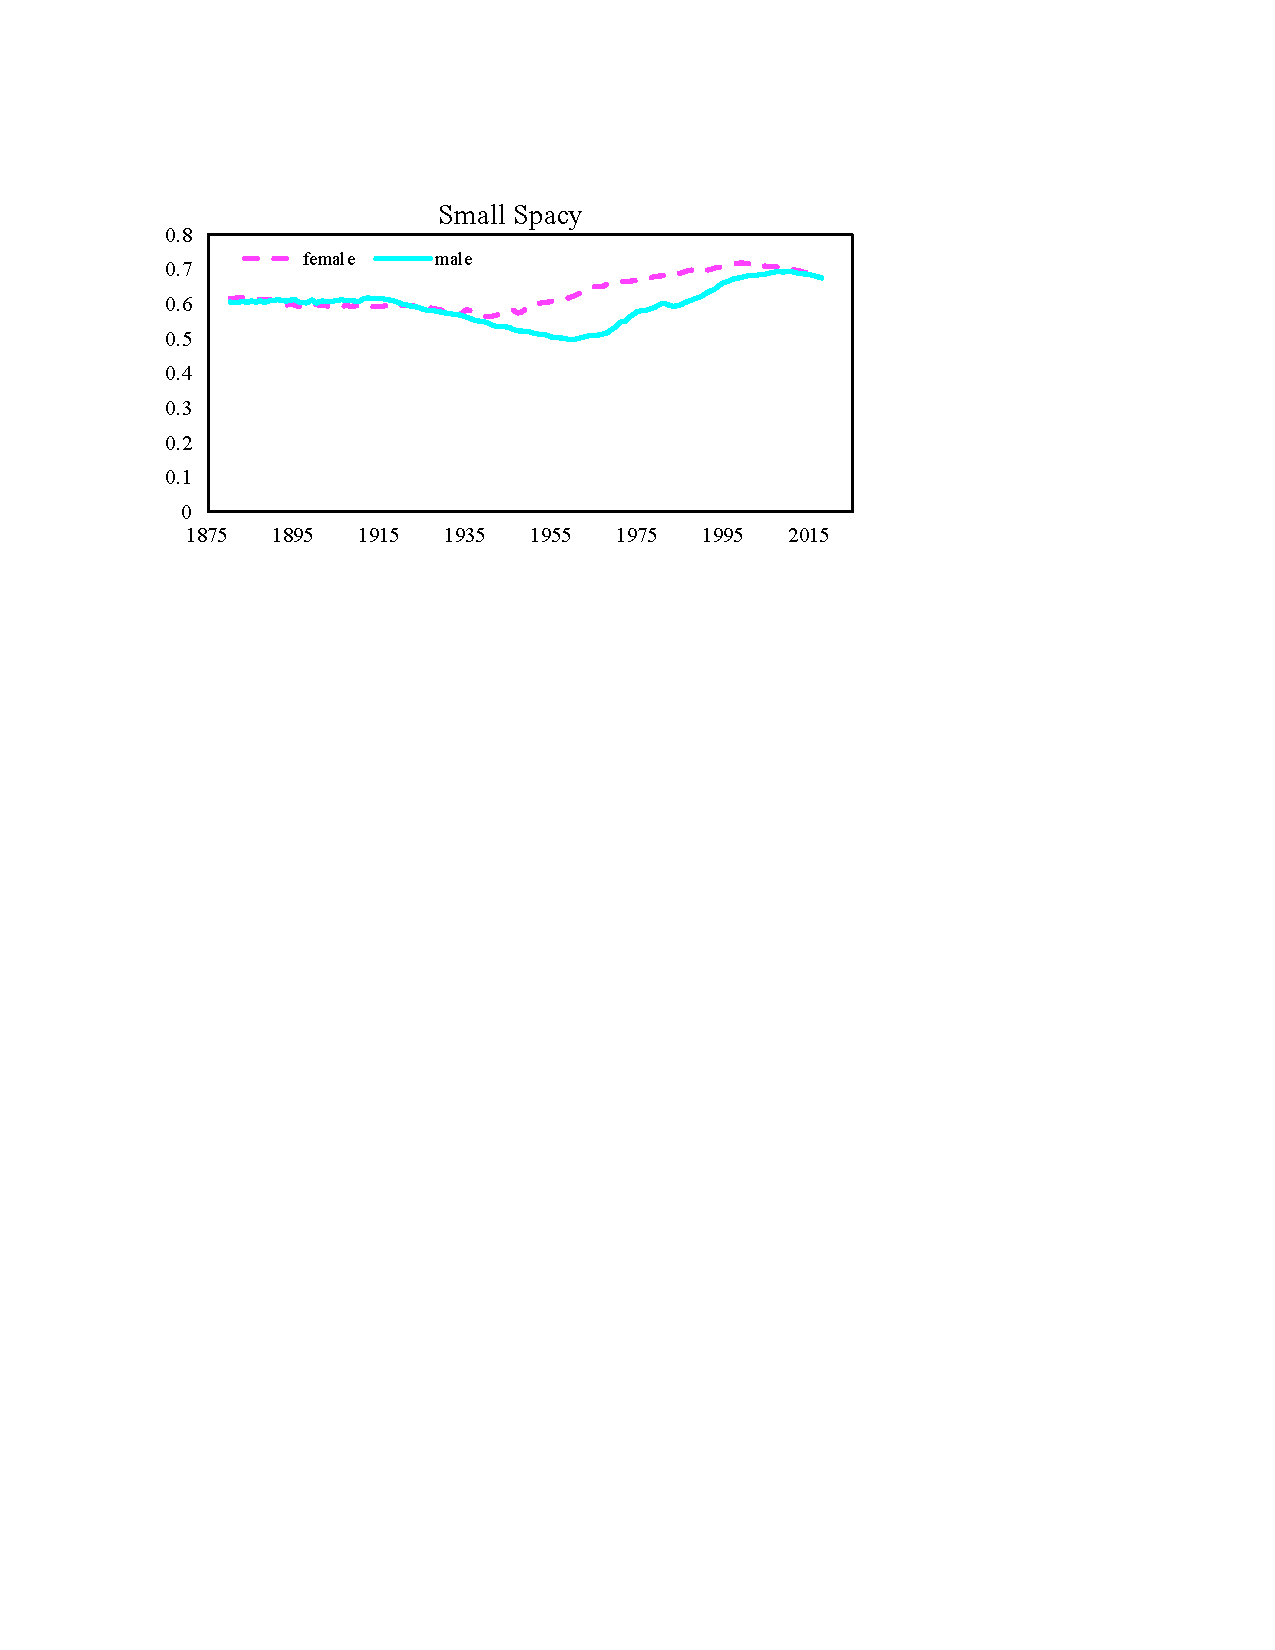
\includegraphics[width=\textwidth,height=0.5\textwidth,trim=0cm 0cm 0cm 0cm,clip=true]{./images/weighted_type2/weighted_type2_2.pdf}
\end{subfigure}
\begin{subfigure}[b]{0.33\textwidth}
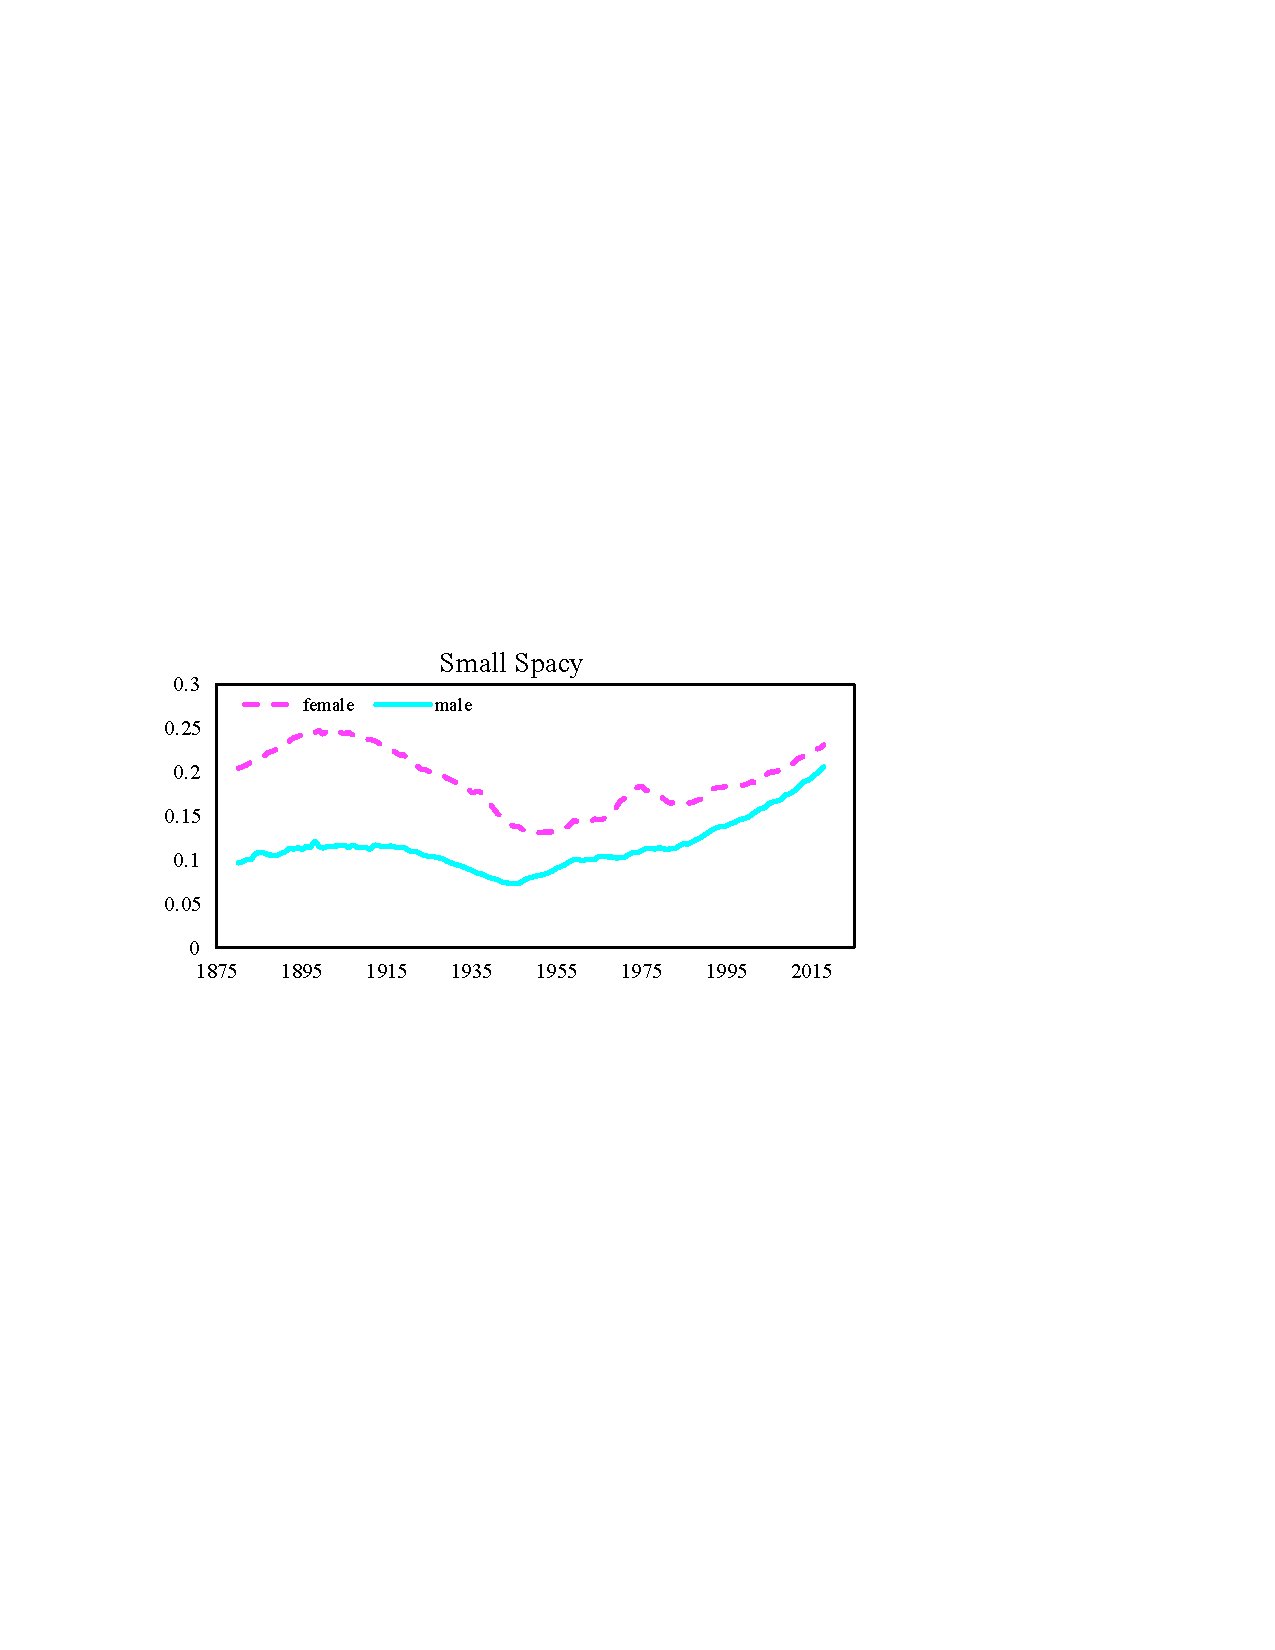
\includegraphics[width=\textwidth,height=0.5\textwidth,trim=0cm 0cm 0cm 0cm,clip=true]{./images/weighted_type3/weighted_type3_2.pdf}
\end{subfigure}
\begin{subfigure}[b]{0.33\textwidth}
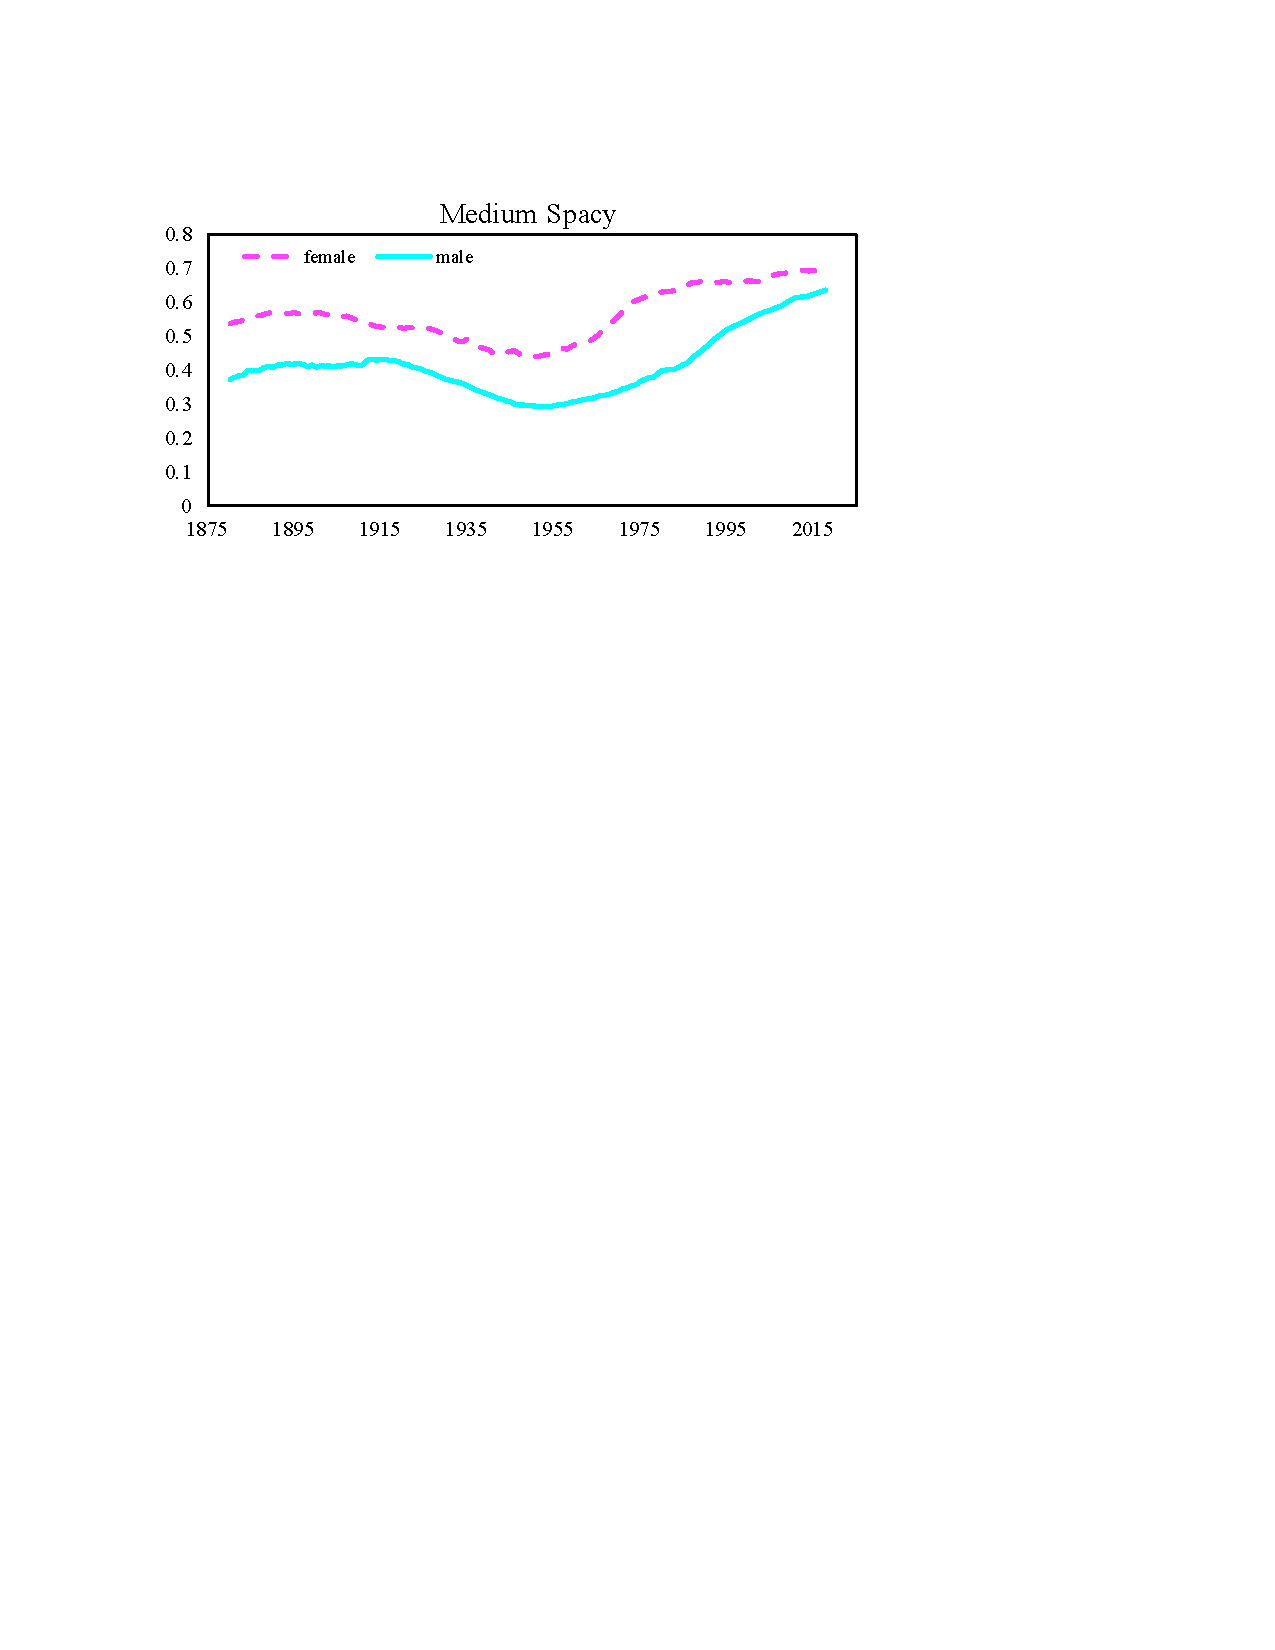
\includegraphics[width=\textwidth,height=0.5\textwidth,trim=0cm 0cm 0cm 0cm,clip=true]{./images/weighted_type1/weighted_type1_3.pdf}
\end{subfigure}
\begin{subfigure}[b]{0.33\textwidth}
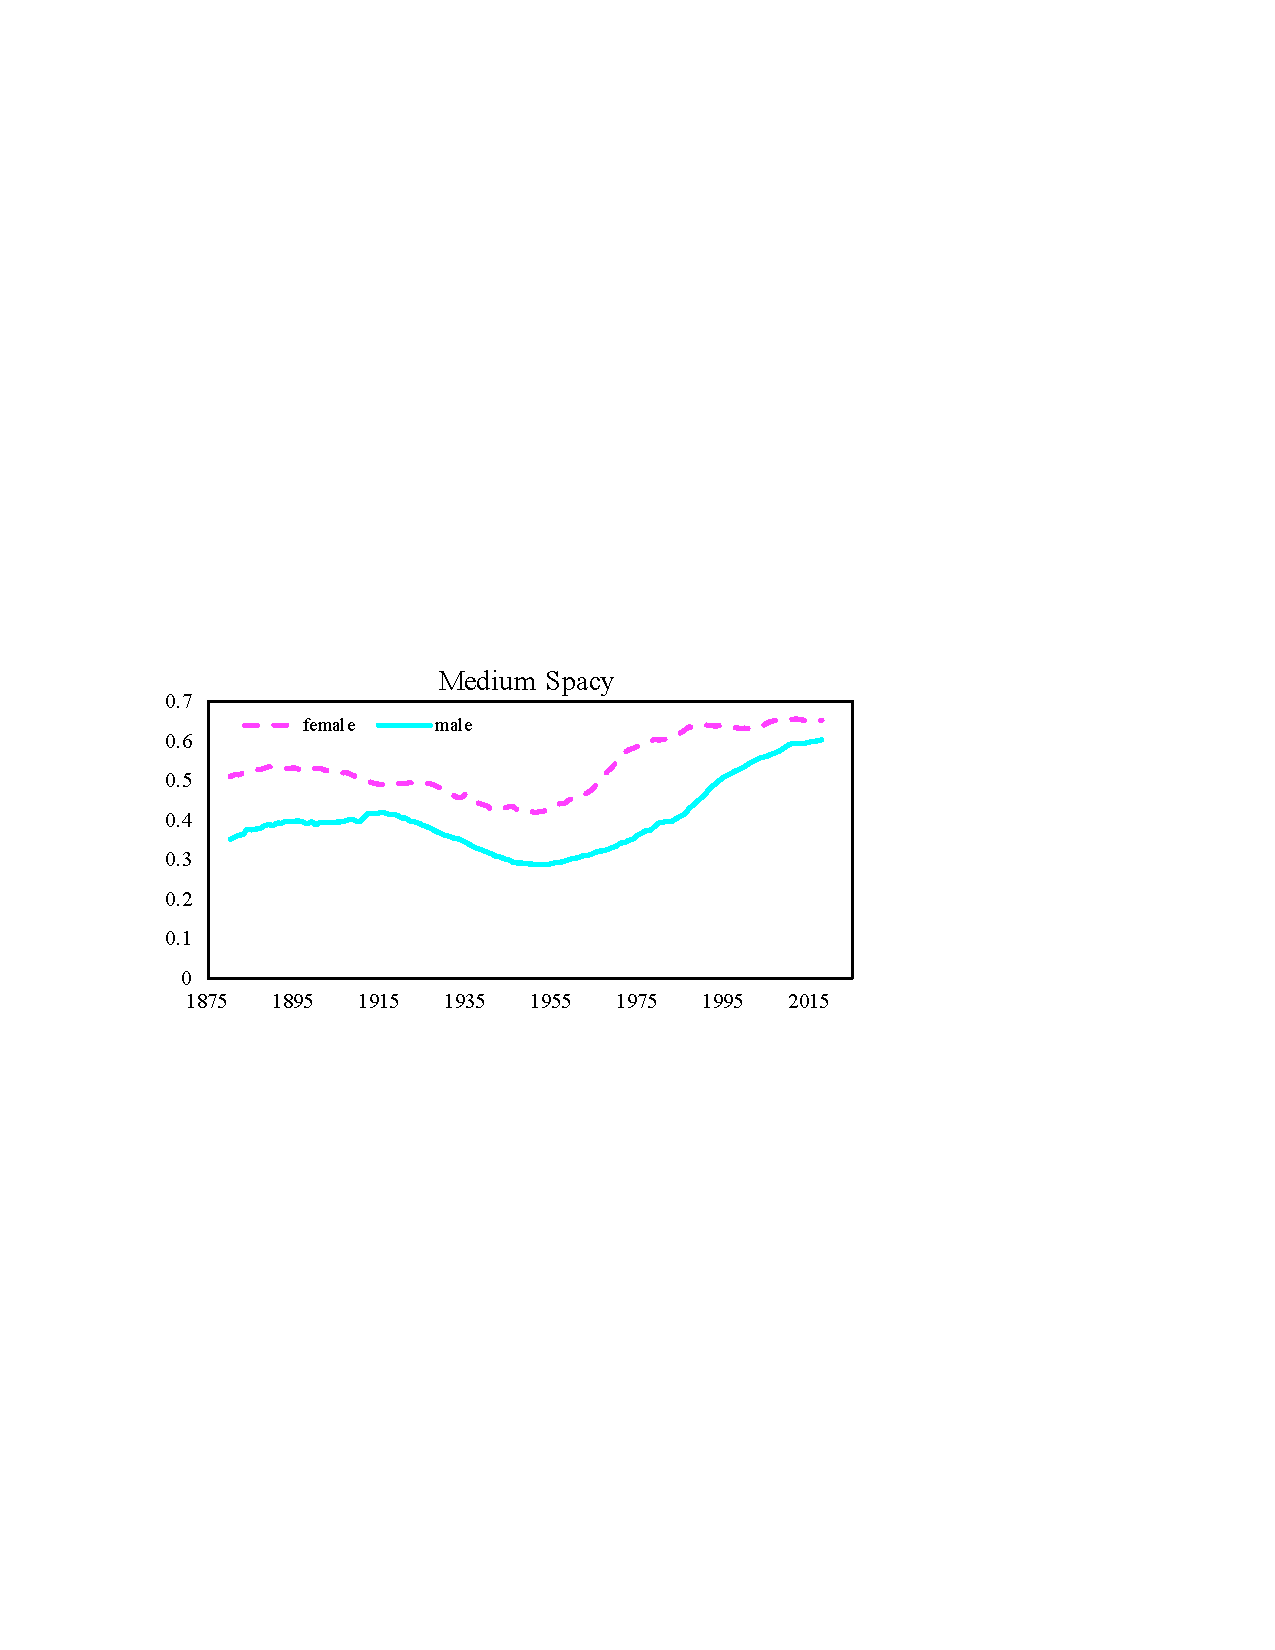
\includegraphics[width=\textwidth,height=0.5\textwidth,trim=0cm 0cm 0cm 0cm,clip=true]{./images/weighted_type2/weighted_type2_3.pdf}
\end{subfigure}
\begin{subfigure}[b]{0.33\textwidth}
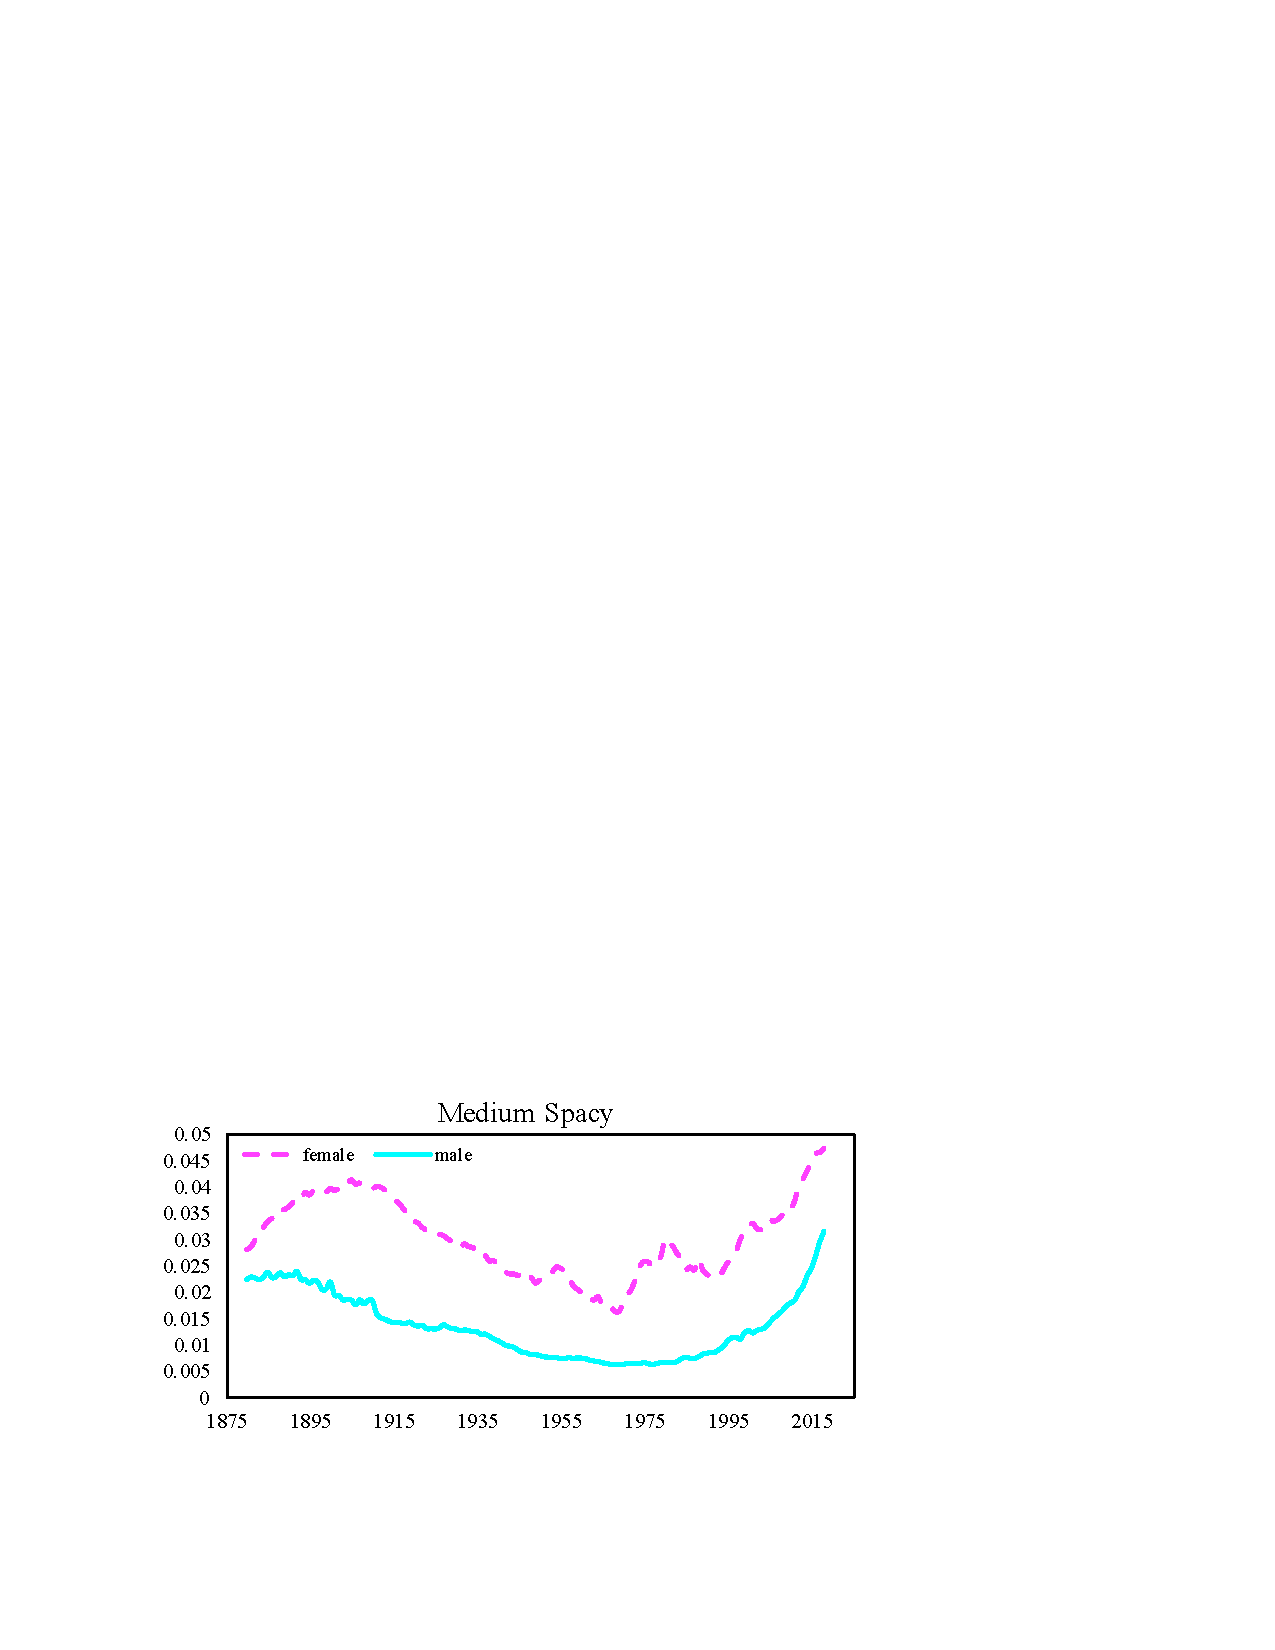
\includegraphics[width=\textwidth,height=0.5\textwidth,trim=0cm 0cm 0cm 0cm,clip=true]{./images/weighted_type3/weighted_type3_3.pdf}
\end{subfigure}
\begin{subfigure}[b]{0.33\textwidth}
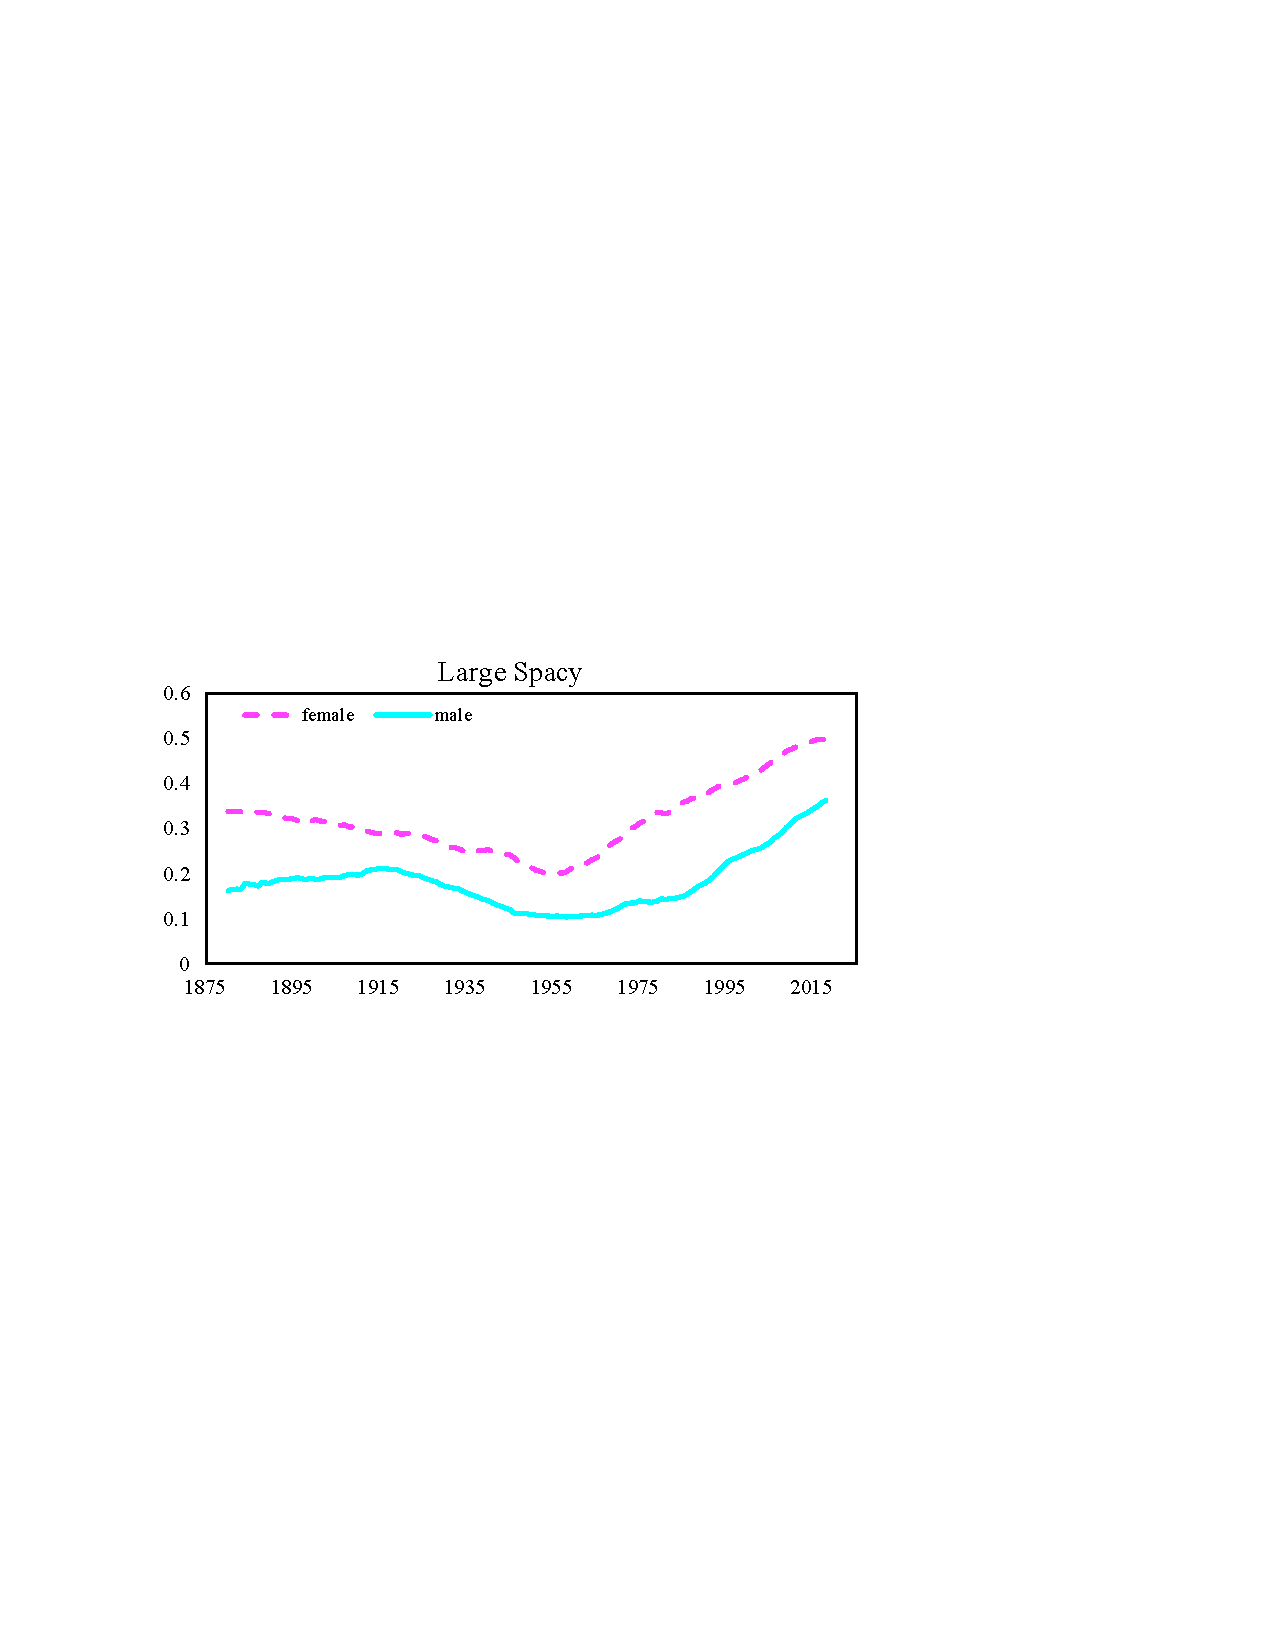
\includegraphics[width=\textwidth,height=0.5\textwidth,trim=0cm 0cm 0cm 0cm,clip=true]{./images/weighted_type1/weighted_type1_4.pdf}
\end{subfigure}
\begin{subfigure}[b]{0.33\textwidth}
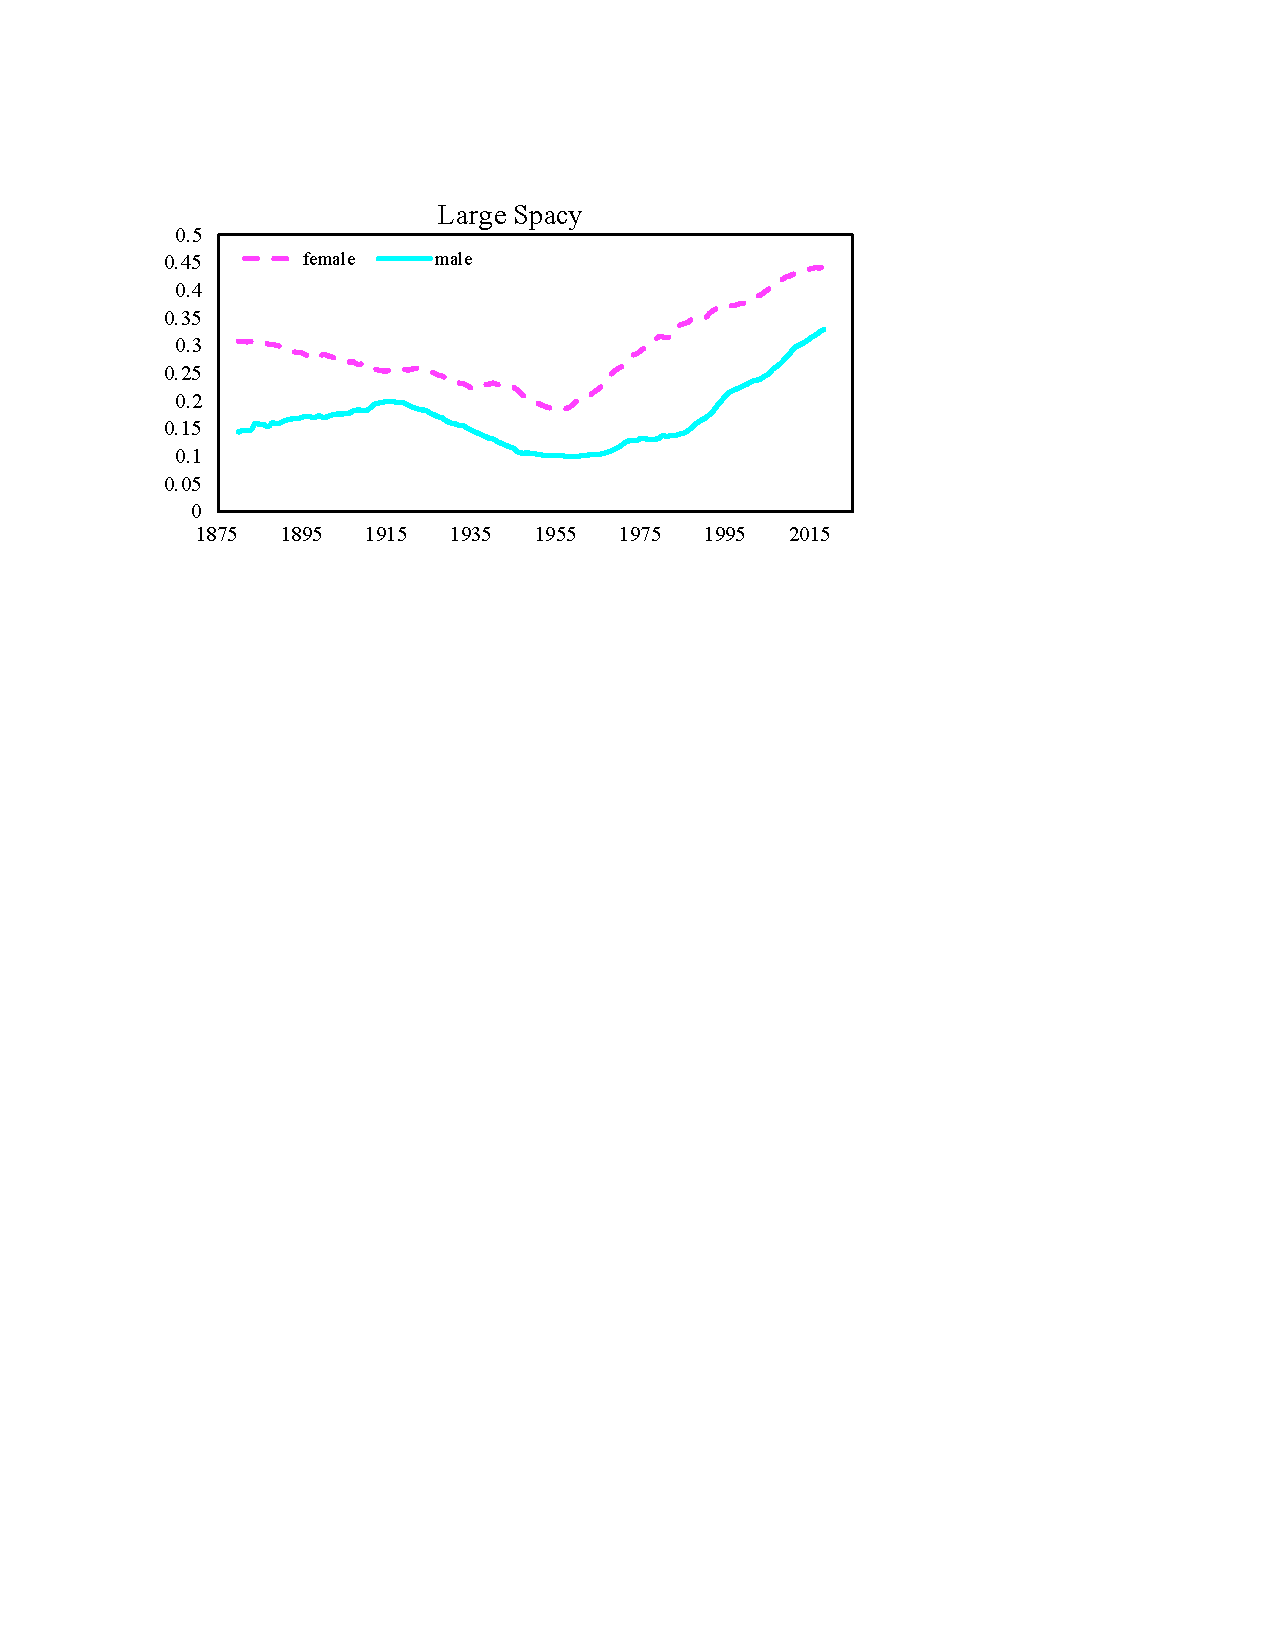
\includegraphics[width=\textwidth,height=0.5\textwidth,trim=0cm 0cm 0cm 0cm,clip=true]{./images/weighted_type2/weighted_type2_4.pdf}
\end{subfigure}
\begin{subfigure}[b]{0.33\textwidth}
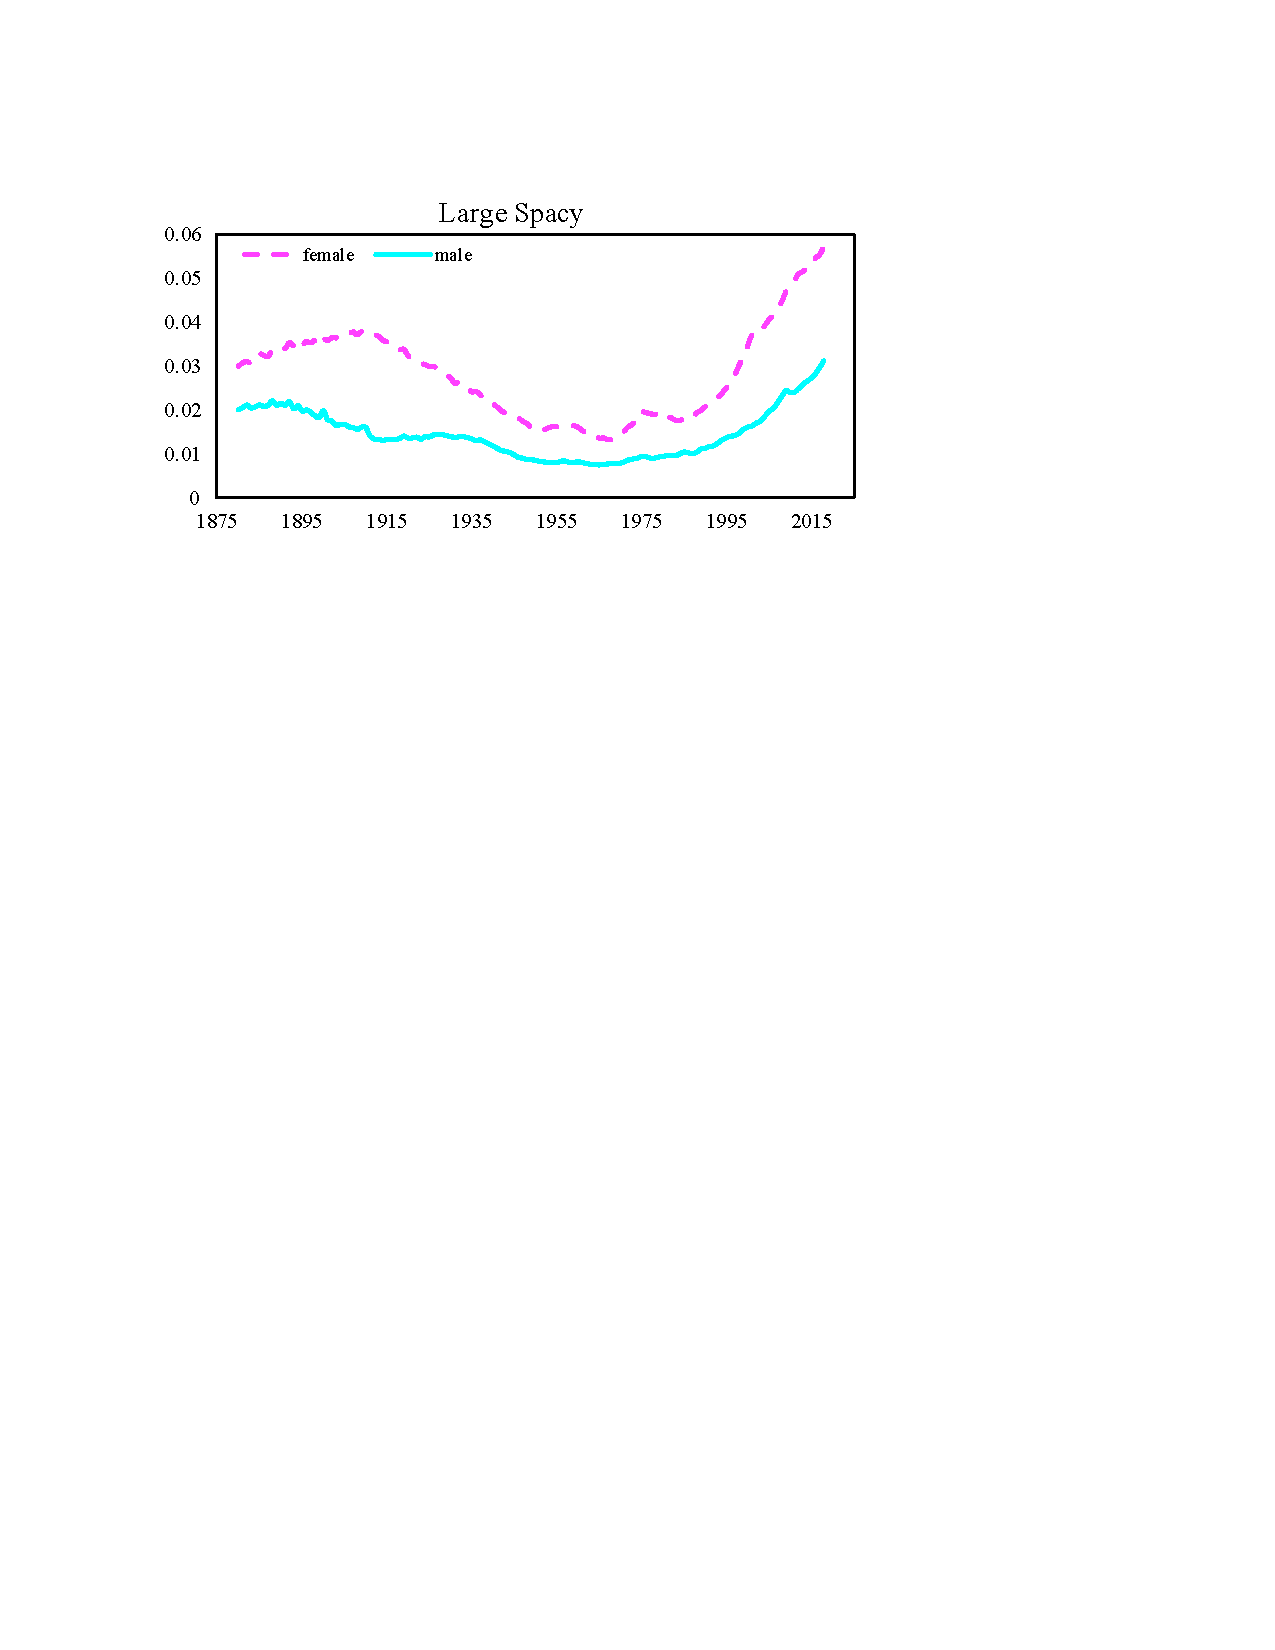
\includegraphics[width=\textwidth,height=0.5\textwidth,trim=0cm 0cm 0cm 0cm,clip=true]{./images/weighted_type3/weighted_type3_4.pdf}
\end{subfigure}
\begin{subfigure}[b]{0.33\textwidth}
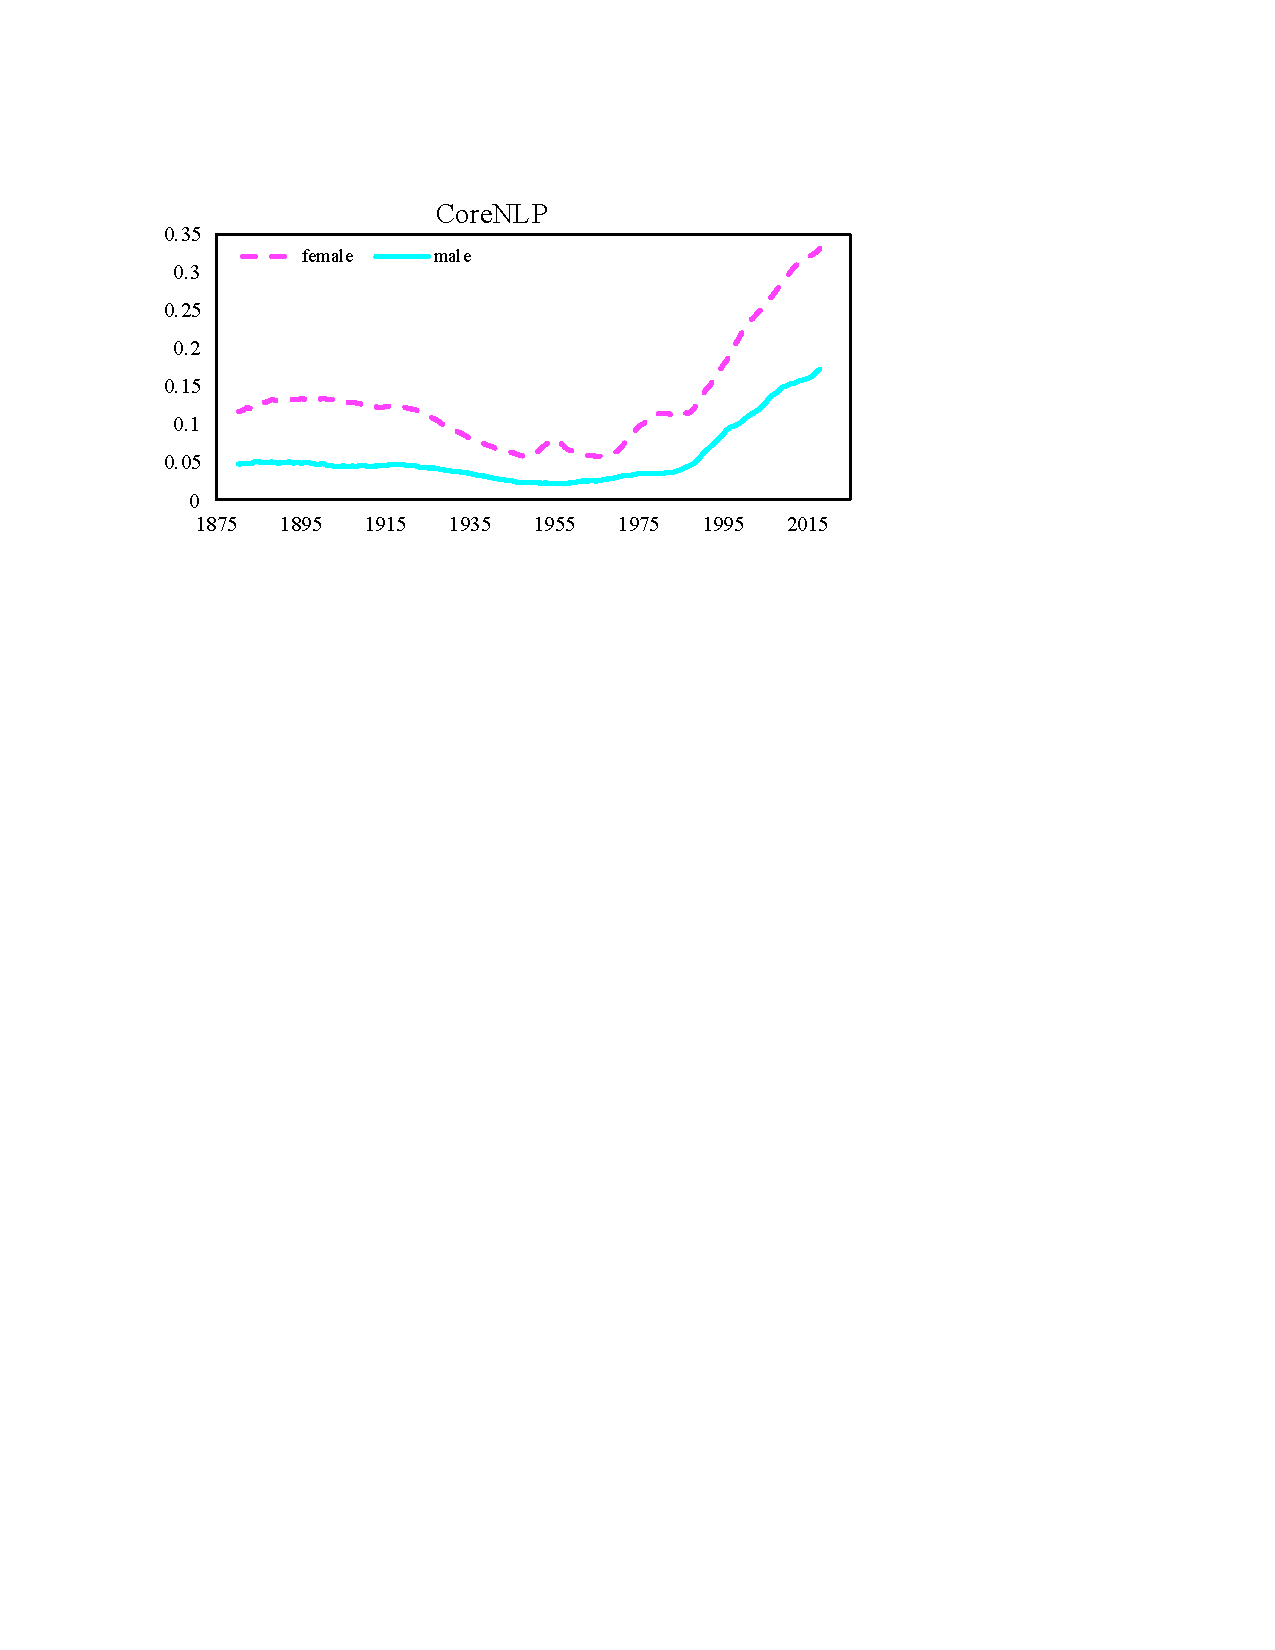
\includegraphics[width=\textwidth,height=0.5\textwidth,trim=0cm 0cm 0cm 0cm,clip=true]{./images/weighted_type1/weighted_type1_5.pdf}
\end{subfigure}
\begin{subfigure}[b]{0.33\textwidth}
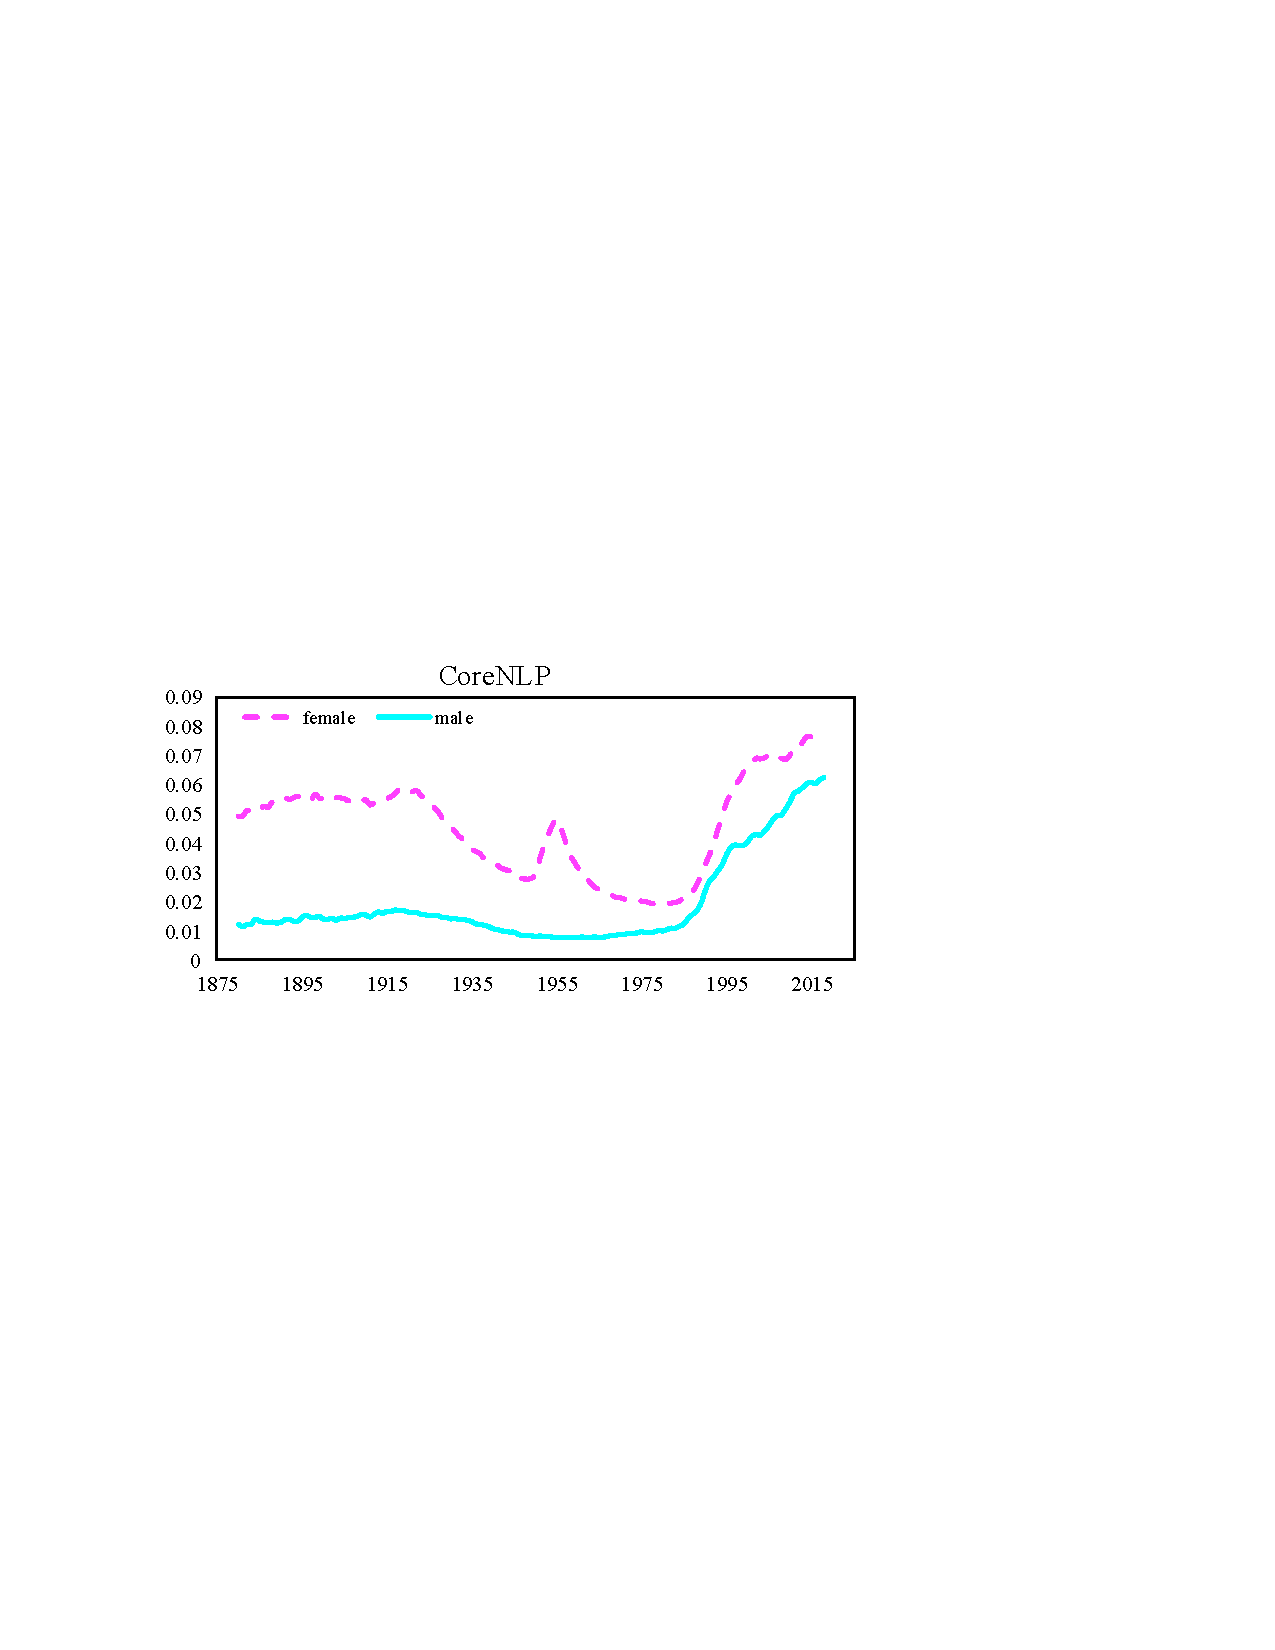
\includegraphics[width=\textwidth,height=0.5\textwidth,trim=0cm 0cm 0cm 0cm,clip=true]{./images/weighted_type2/weighted_type2_5.pdf}
\end{subfigure}
\begin{subfigure}[b]{0.33\textwidth}
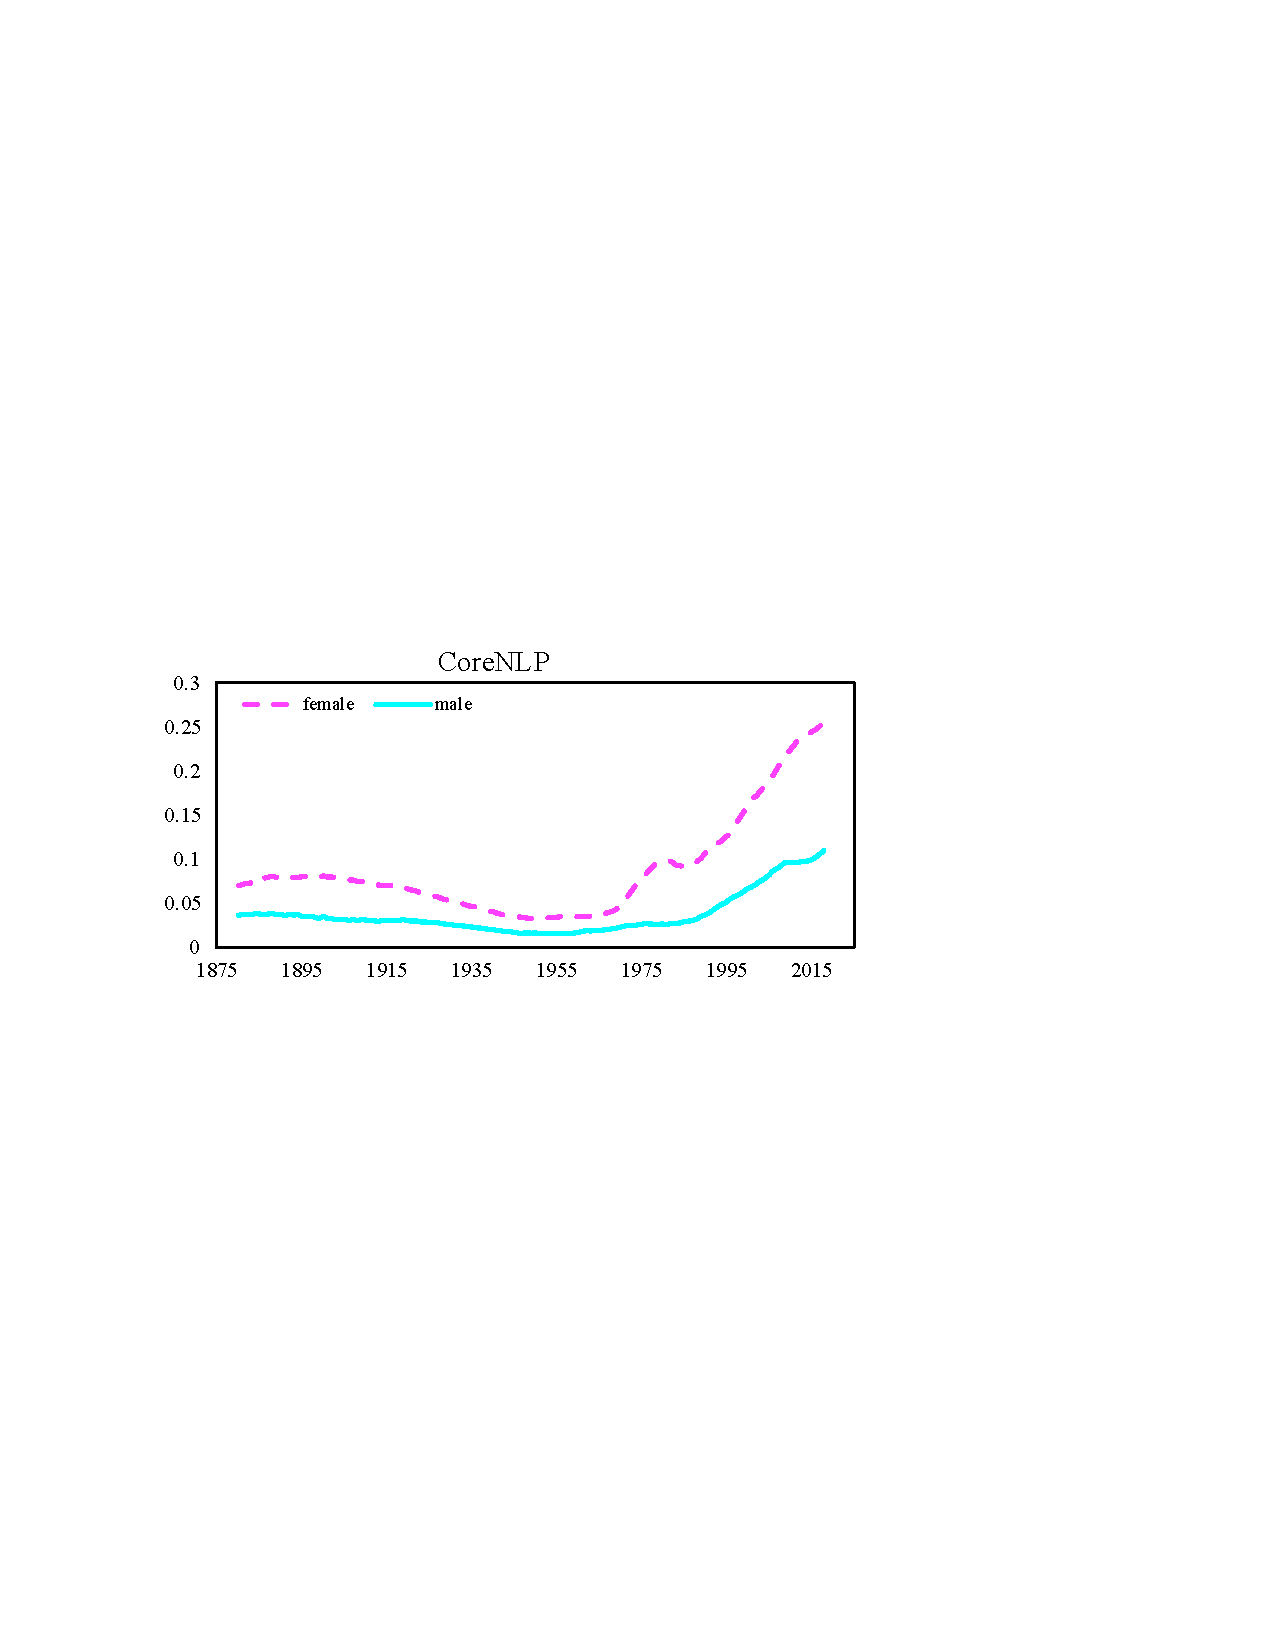
\includegraphics[width=\textwidth,height=0.5\textwidth,trim=0cm 0cm 0cm 0cm,clip=true]{./images/weighted_type3/weighted_type3_5.pdf}
\end{subfigure}
\caption{Results from different models that spanned the 139-year history of baby names from the census data on different error types for the weighted cases using template \#4. Female names have higher error rates for all the cases. The y axis shows the calculated error rates for each of the error types as described in their corresponding formulas, and the x axis represents the year in which the baby name was given.}
\label{result1}
\end{figure*}
\subsection{Experimental Design and Results}
\begin{table}
\centering
\begin{tabular}{ p{1cm}p{5.0cm}}
 \toprule
\#&Template Sentence\\
 \midrule
 1&\textbf{\textless Name\textgreater}\\[0.5pt]
 2&\textbf{\textless Name\textgreater} is going to school\\[0.5pt]
 3&\textbf{\textless Name\textgreater} is at school\\[0.5pt]
 4&\textbf{\textless Name\textgreater} is a person\\[0.5pt]
 5&\textbf{\textless Name\textgreater} is eating food\\[0.5pt]
 6&\textbf{\textless Name\textgreater} is going to grocery shop\\[0.5pt]
 7&\textbf{\textless Name\textgreater} is going to work\\[0.5pt]
 8&\textbf{\textless Name\textgreater} is a nurse\\[0.5pt]
 9&\textbf{\textless Name\textgreater} is a doctor\\[0.5pt]
 \bottomrule
\end{tabular}
\caption{Templates that form our benchmark with their corresponding numbers as referenced in the paper. Template 1 is the ``no context'' template.}
\label{Templates}
\end{table}
We ran each NER model on our created benchmark dataset, for all 139 years, and analyzed the performance of each template over female vs. male genders and compared the results of these models across genders per year. We report six sets of results based upon different concepts of error. The different errors we consider are discussed below. $N_f$ is the set of female names in a particular year. The same error is calculated for male using $N_m$ --- the set of male names.

\subsubsection{Error Type-1 Unweighted.} 
This is a type of error that measures names that are tagged as non-PERSON, or not tagged at all. In other words, any name not tagged as a PERSON is considered to be an error.
\[ \frac{\sum_{n \in N_f}I(n_{type} \neq PERSON)}{|N_f|}\]

\subsubsection{Error Type-1 Weighted.} This type of error is similar to Error Type-1 Unweighted; however, we considered how frequent the mistaken name is based on census data while calculating the error.
\[ \frac{\sum_{n \in N_f}freq_f(n_{type} \neq PERSON)}{\sum_{n \in N_f}freq_f(n)},\]
where $freq_f(\cdot)$ returns the frequency of a name in the female census data in a particular year. Similarly, $freq_m(\cdot)$ will yield the frequency of a name in the male census data.
Type-1 errors can be sub-divided into Type-2 and Type-3 errors and serve as a super-set for the following types.
\subsubsection{Error Type-2 Unweighted.} This is a type of error in which only names that are tagged,  but whose tags are non-PERSON are considered to be errors. This measure is similar to precision, where the model is only punished for incorrect retrieval. This error rate reports the percentage of names that are tagged as non-PERSON entities among all the names in a certain year.
\[ \frac{\sum_{n \in N_f}I(n_{type} \notin \{\emptyset,PERSON\})}{|N_f|},\]
where $\emptyset$ indicates the name is not tagged.
\subsubsection{Error Type-2 Weighted.} This type of error is similar to Error Type-2 Unweighted; however, here we considered how frequent the mistaken name was while calculating the error.
\[ \frac{\sum_{n \in N_f}freq_f(n_{type} \notin \{\emptyset,PERSON\})}{\sum_{n \in N_f}freq_f(n)}\]

\subsubsection{Error Type-3 Unweighted.} This is a type of error in which only names that are not tagged are considered to be errors. We do not consider names that are wrongfully tagged to non-PERSON as an error, but only names that are not tagged are considered erroneous. This error rate reports the percentage of names that are not tagged at all among all the names in a certain year.
\[ \frac{\sum_{n \in N_f}I(n_{type} = \emptyset)}{|N_f|}\]

\subsubsection{Error Type-3 Weighted.} This type of error is similar to Error Type-3 Unweighted; however, we considered how frequent the mistaken name was while calculating the error.
\[ \frac{\sum_{n \in N_f}freq_f(n_{type} = \emptyset)}{\sum_{n \in N_f}freq_f(n)}\]
% \begin{figure*}[!bt]
% 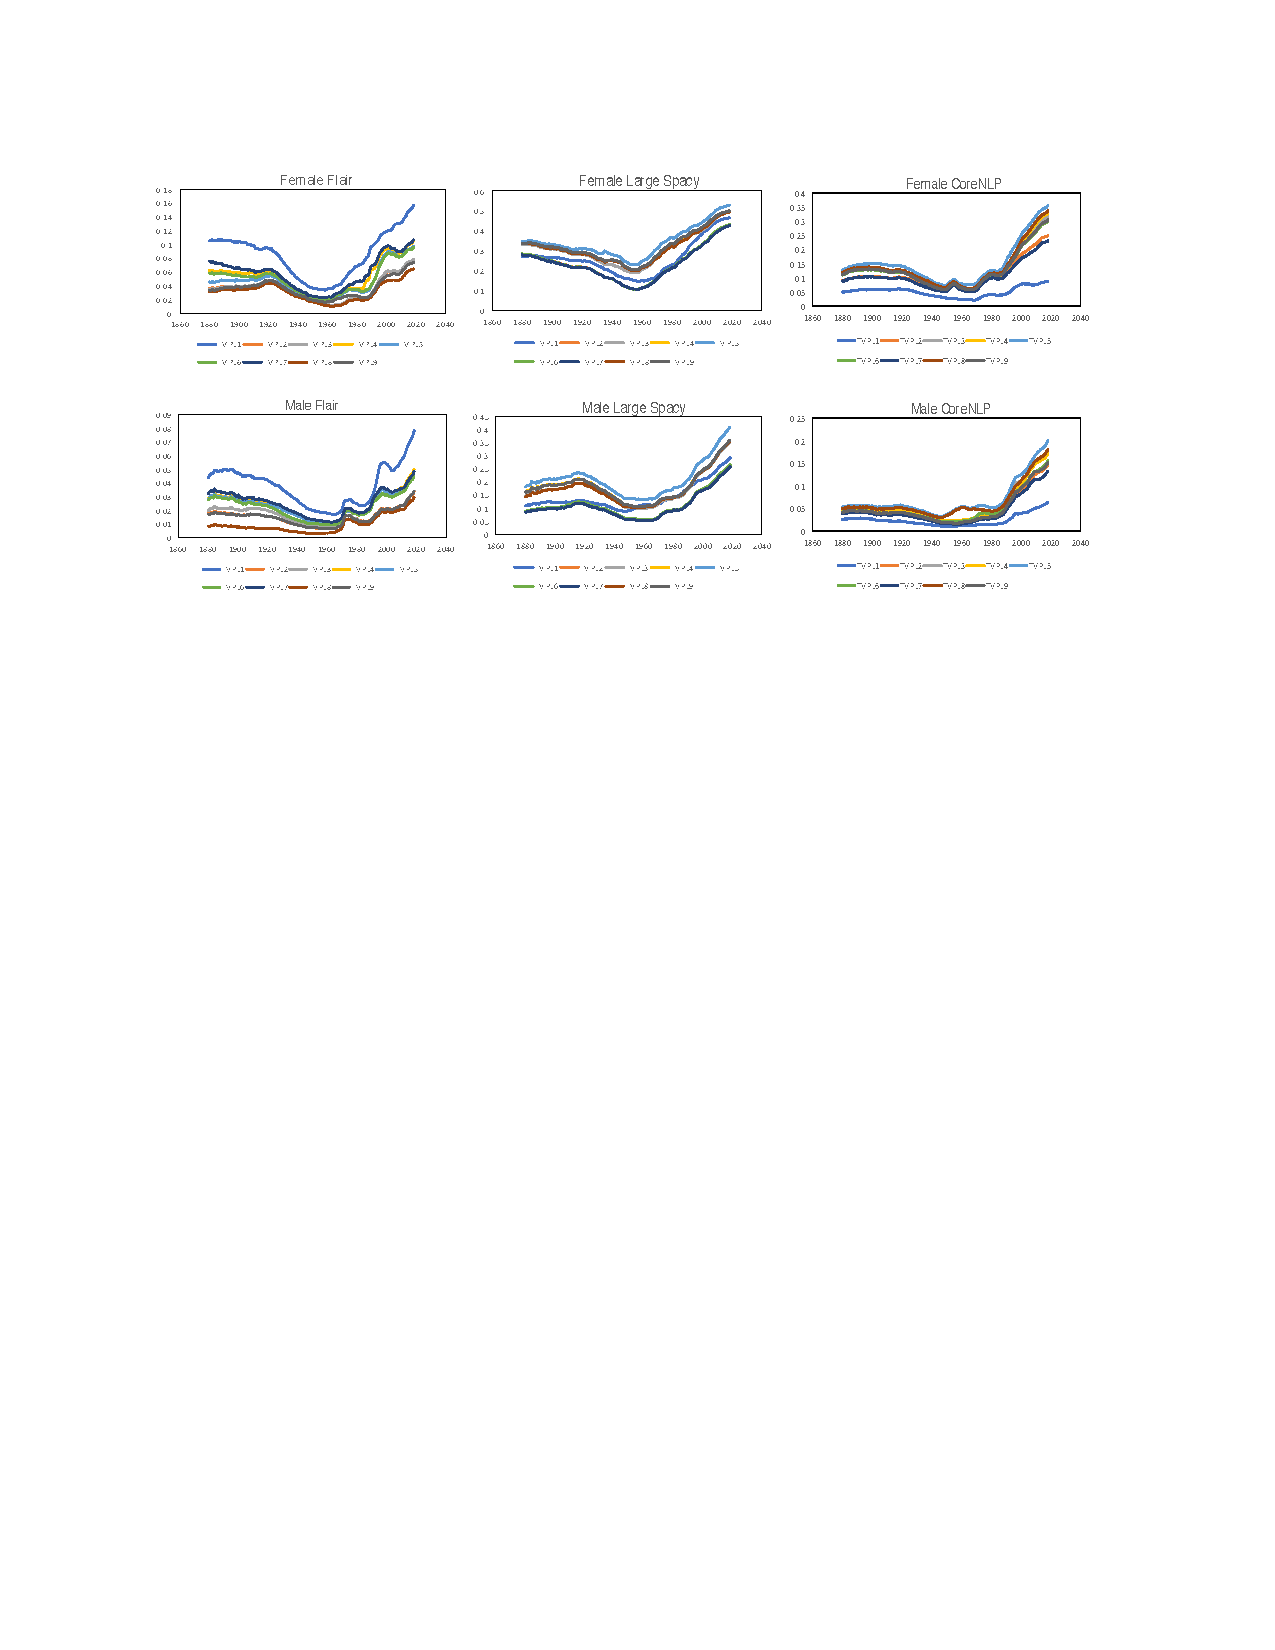
\includegraphics[width=\textwidth,height=0.4\textwidth,trim=0cm 0cm 0cm 0cm,clip=true]{templates2.pdf}
% \caption{Performance of different models on different templates from our benchmark for female and male names over 139 years. Notice how context in some of the templates helped some models, while had negative effects on some other models.}
% \label{tempresults}
% \end{figure*}
\begin{figure*}[!bt]
% \includegraphics[width=\textwidth,height=0.9\textwidth,trim=0.5cm 0.2cm 0.4cm 0cm,clip=true]{results1.pdf}
%\begin{subfigure}[b]{\textwidth}
%\centering
% \includegraphics[width=1\textwidth,height=0.16\textwidth,trim=0cm 0cm 0cm 0cm,clip=true]{weighted_combined.pdf}
\begin{subfigure}[b]{0.33\textwidth}
\caption{Error Type-1 Unweighted}
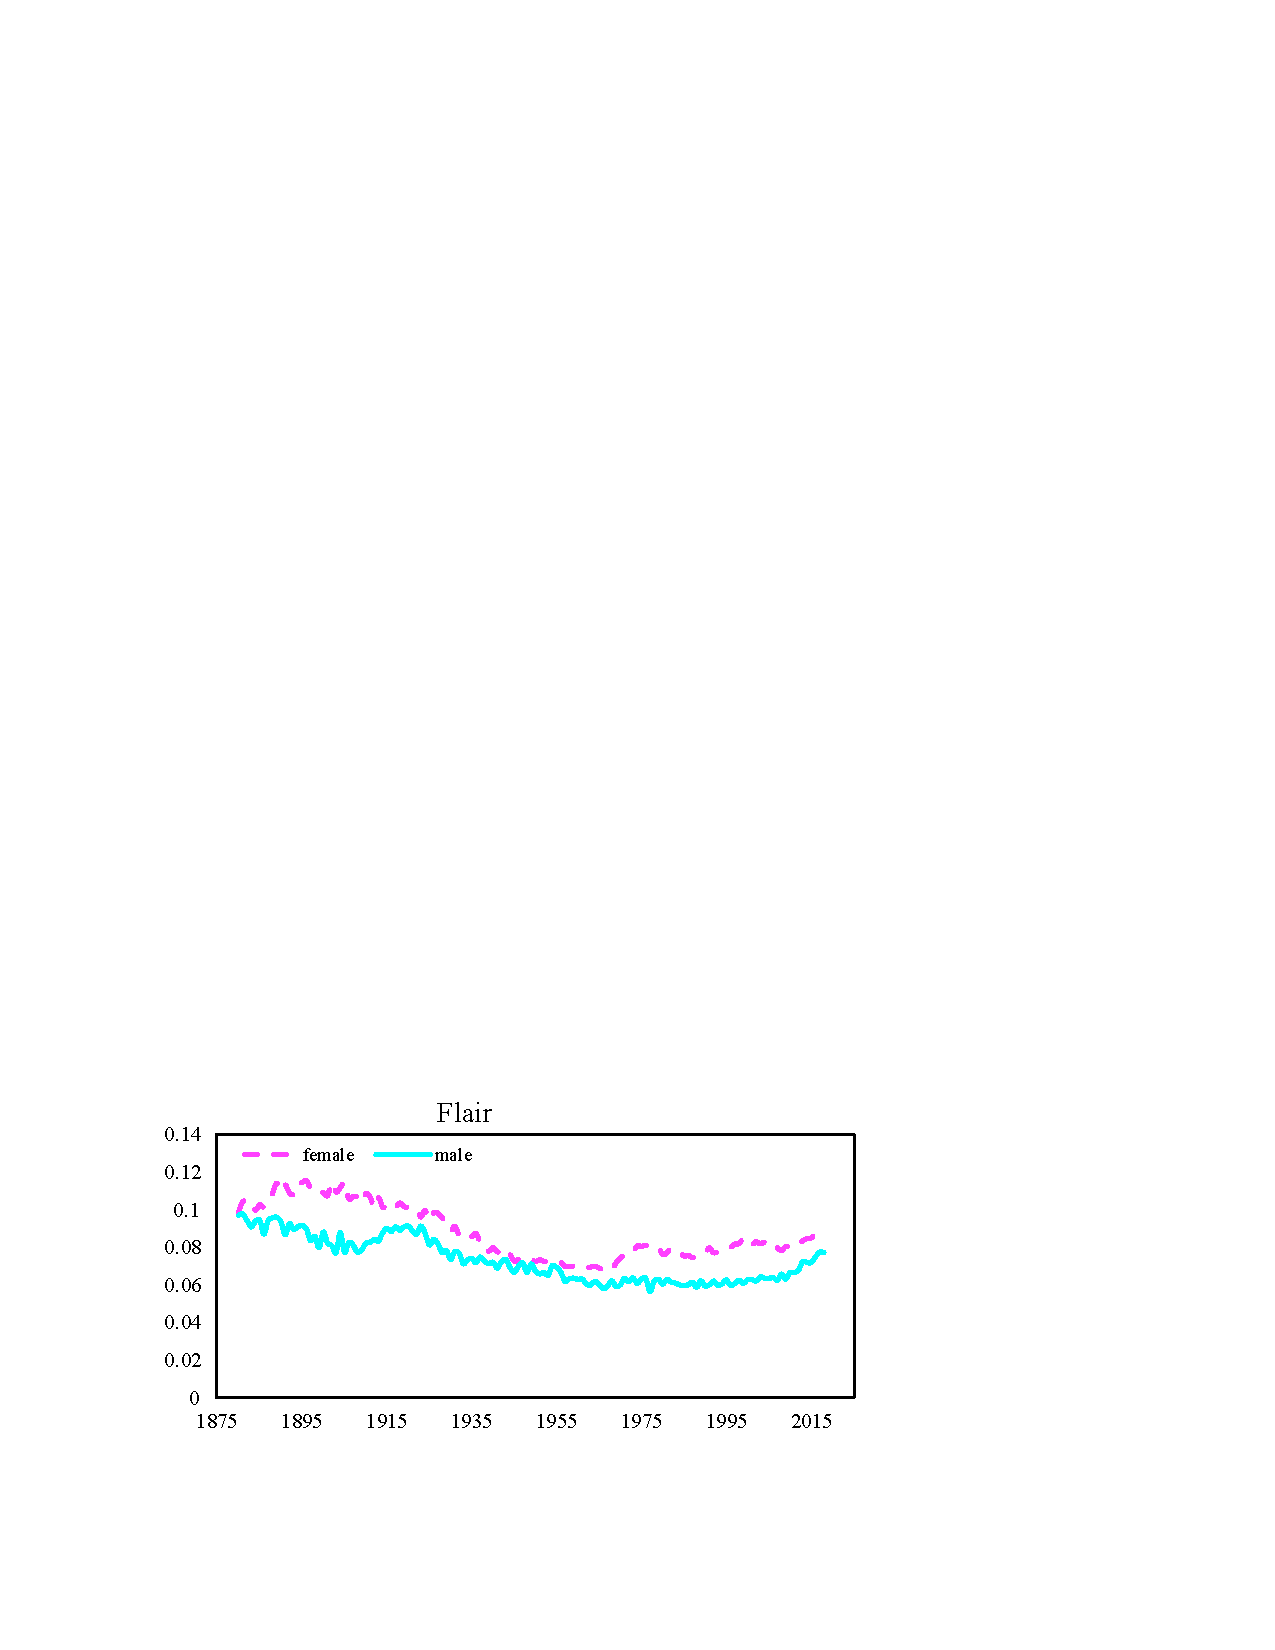
\includegraphics[width=\textwidth,height=0.5\textwidth,trim=0cm 0cm 0cm 0cm,clip=true]{./images/unweighted_type1/unweighted_type1_1.pdf}
\end{subfigure}
\begin{subfigure}[b]{0.33\textwidth}
\caption{Error Type-2 Unweighted}
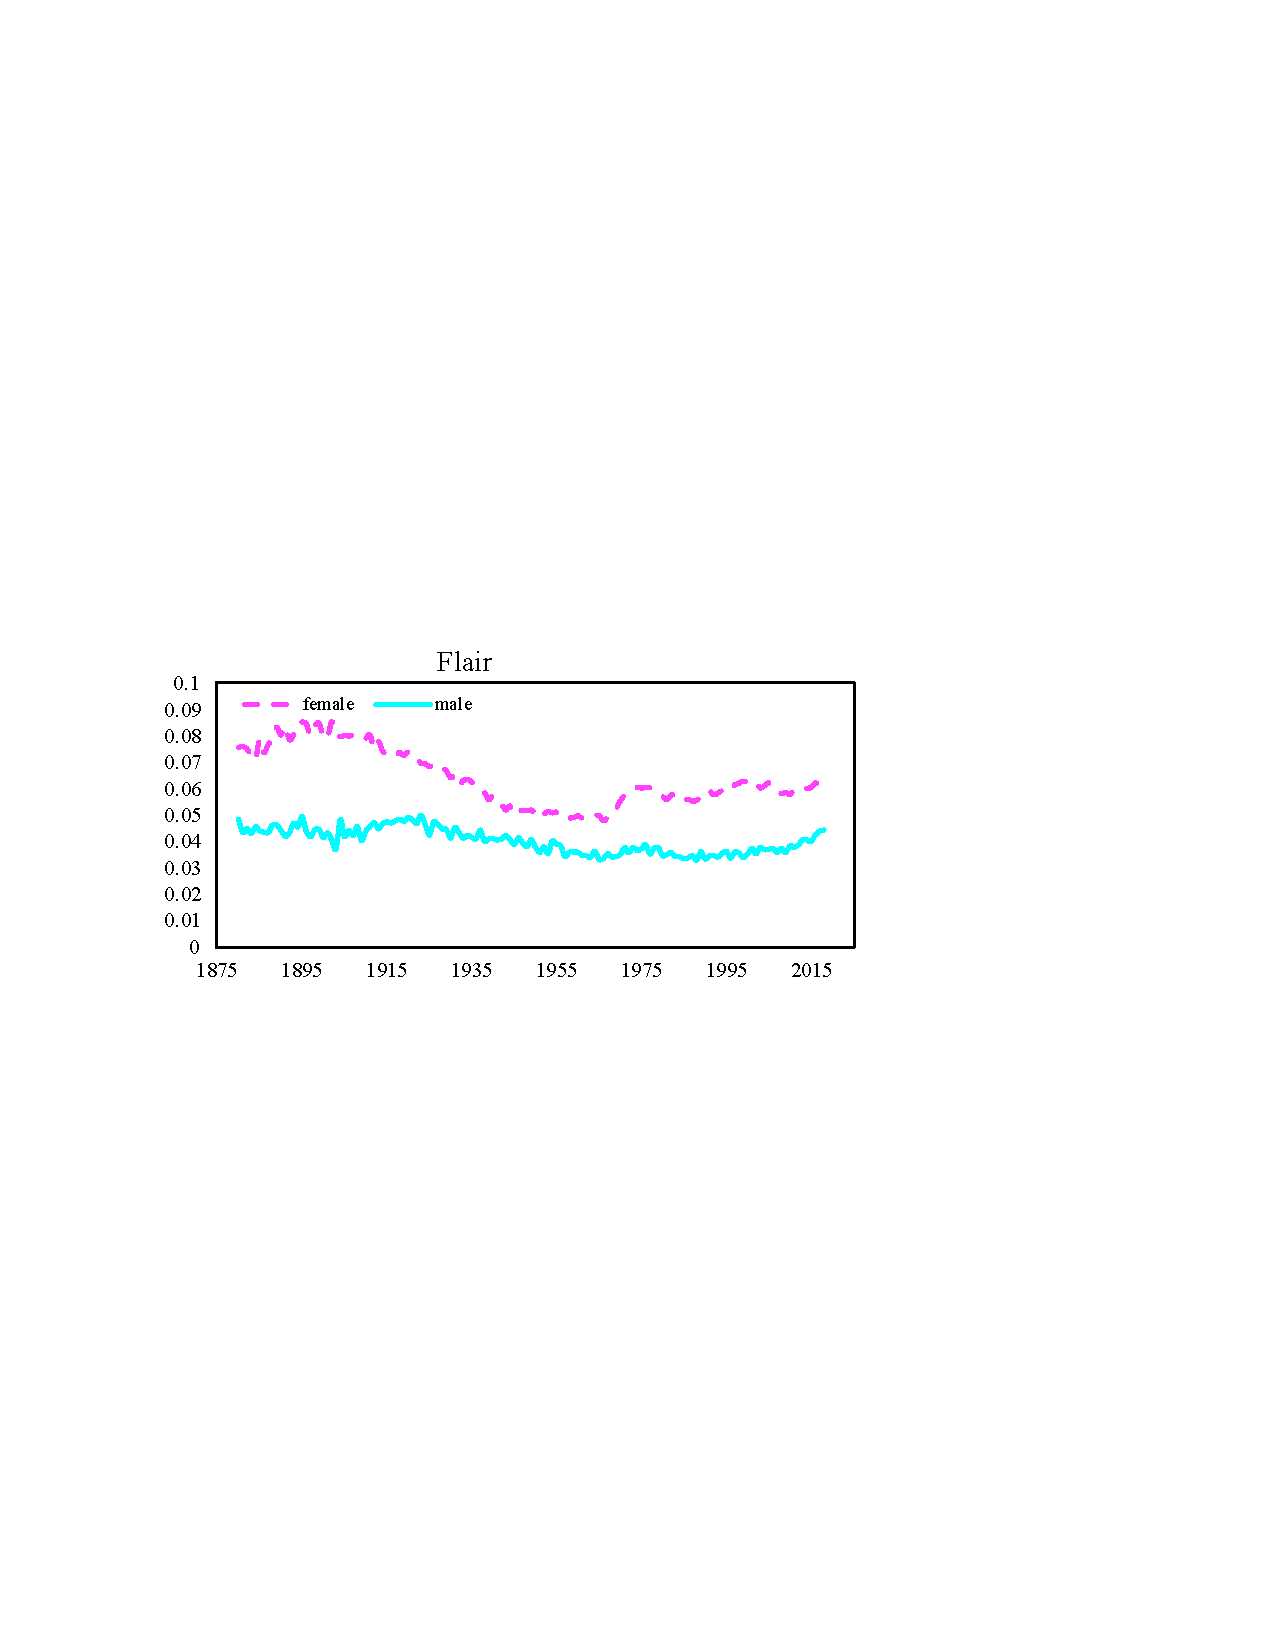
\includegraphics[width=\textwidth,height=0.5\textwidth,trim=0cm 0cm 0cm 0cm,clip=true]{./images/unweighted_type2/unweighted_type2_1.pdf}
\end{subfigure}
\begin{subfigure}[b]{0.33\textwidth}
\caption{Error Type-3 Unweighted}
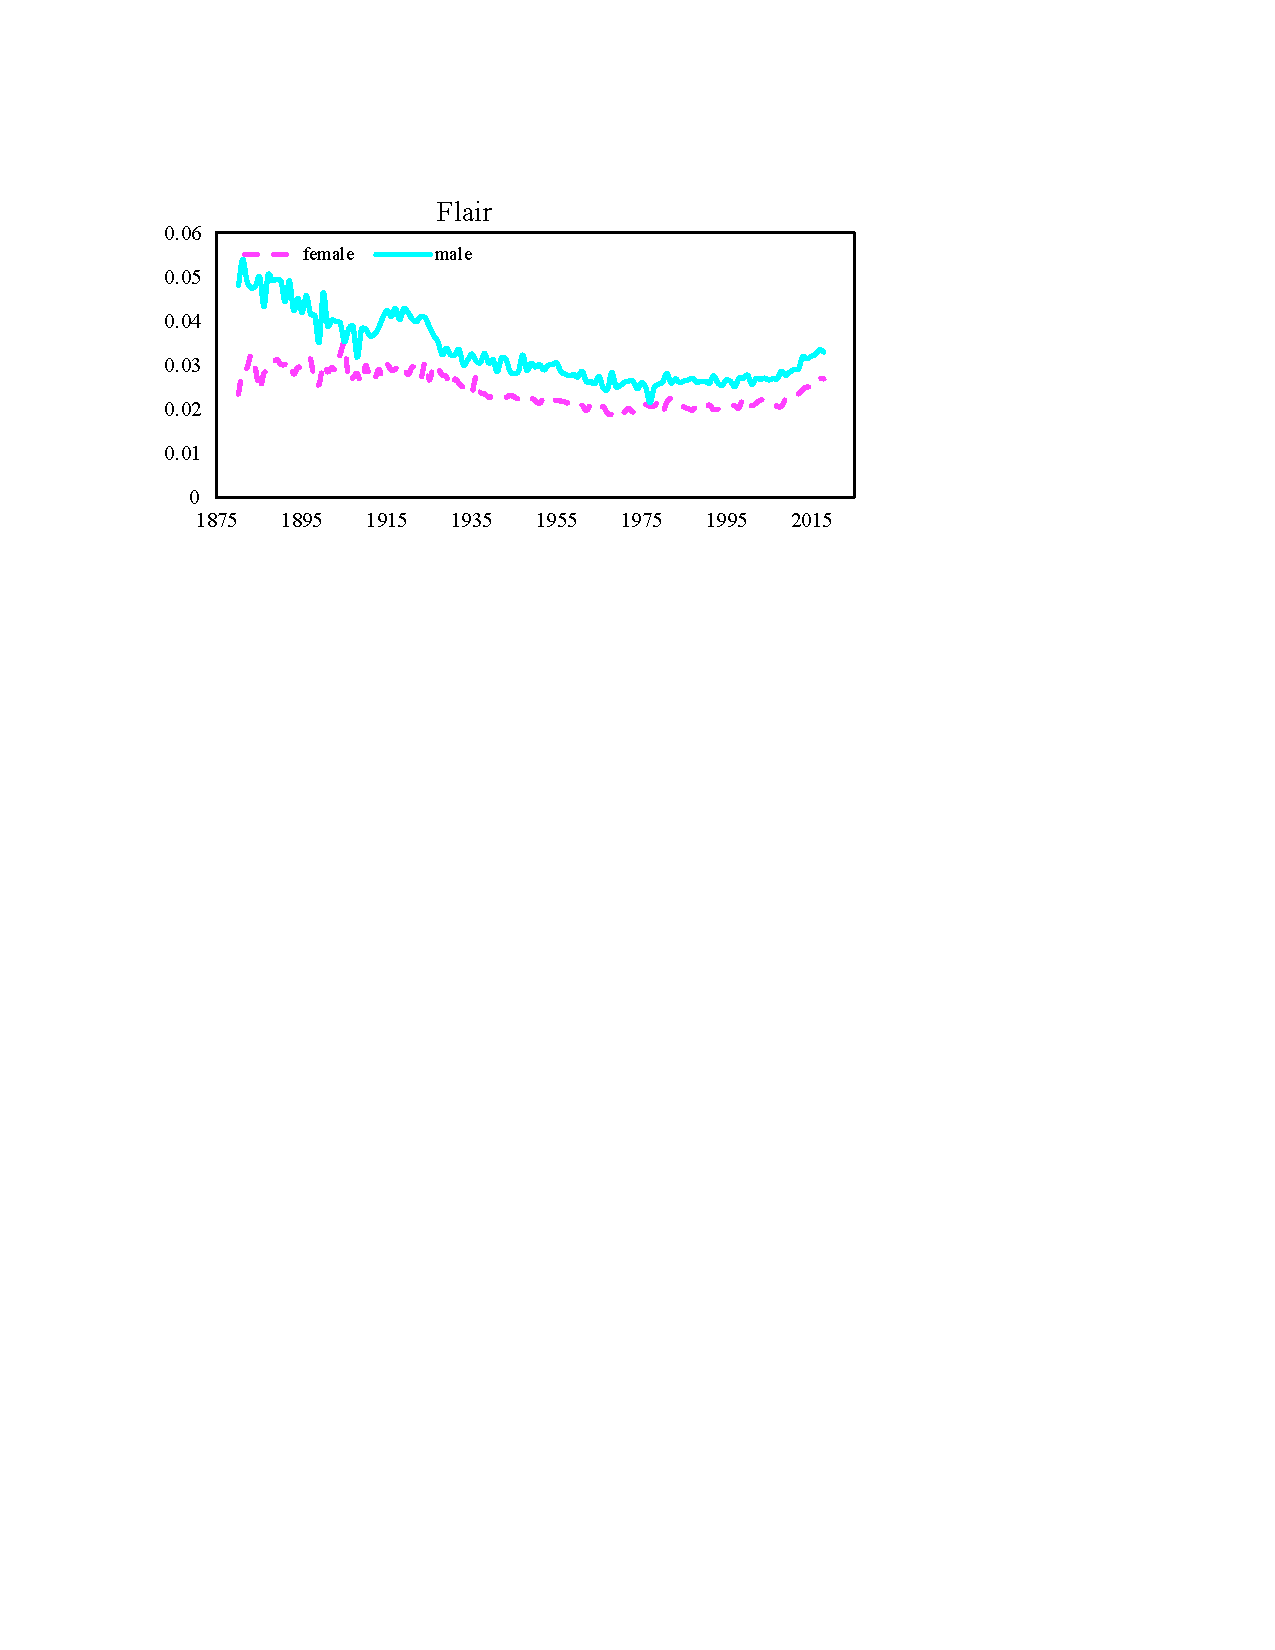
\includegraphics[width=\textwidth,height=0.5\textwidth,trim=0cm 0cm 0cm 0cm,clip=true]{./images/unweighted_type3/unweighted_type3_1.pdf}
\end{subfigure}
\begin{subfigure}[b]{0.33\textwidth}
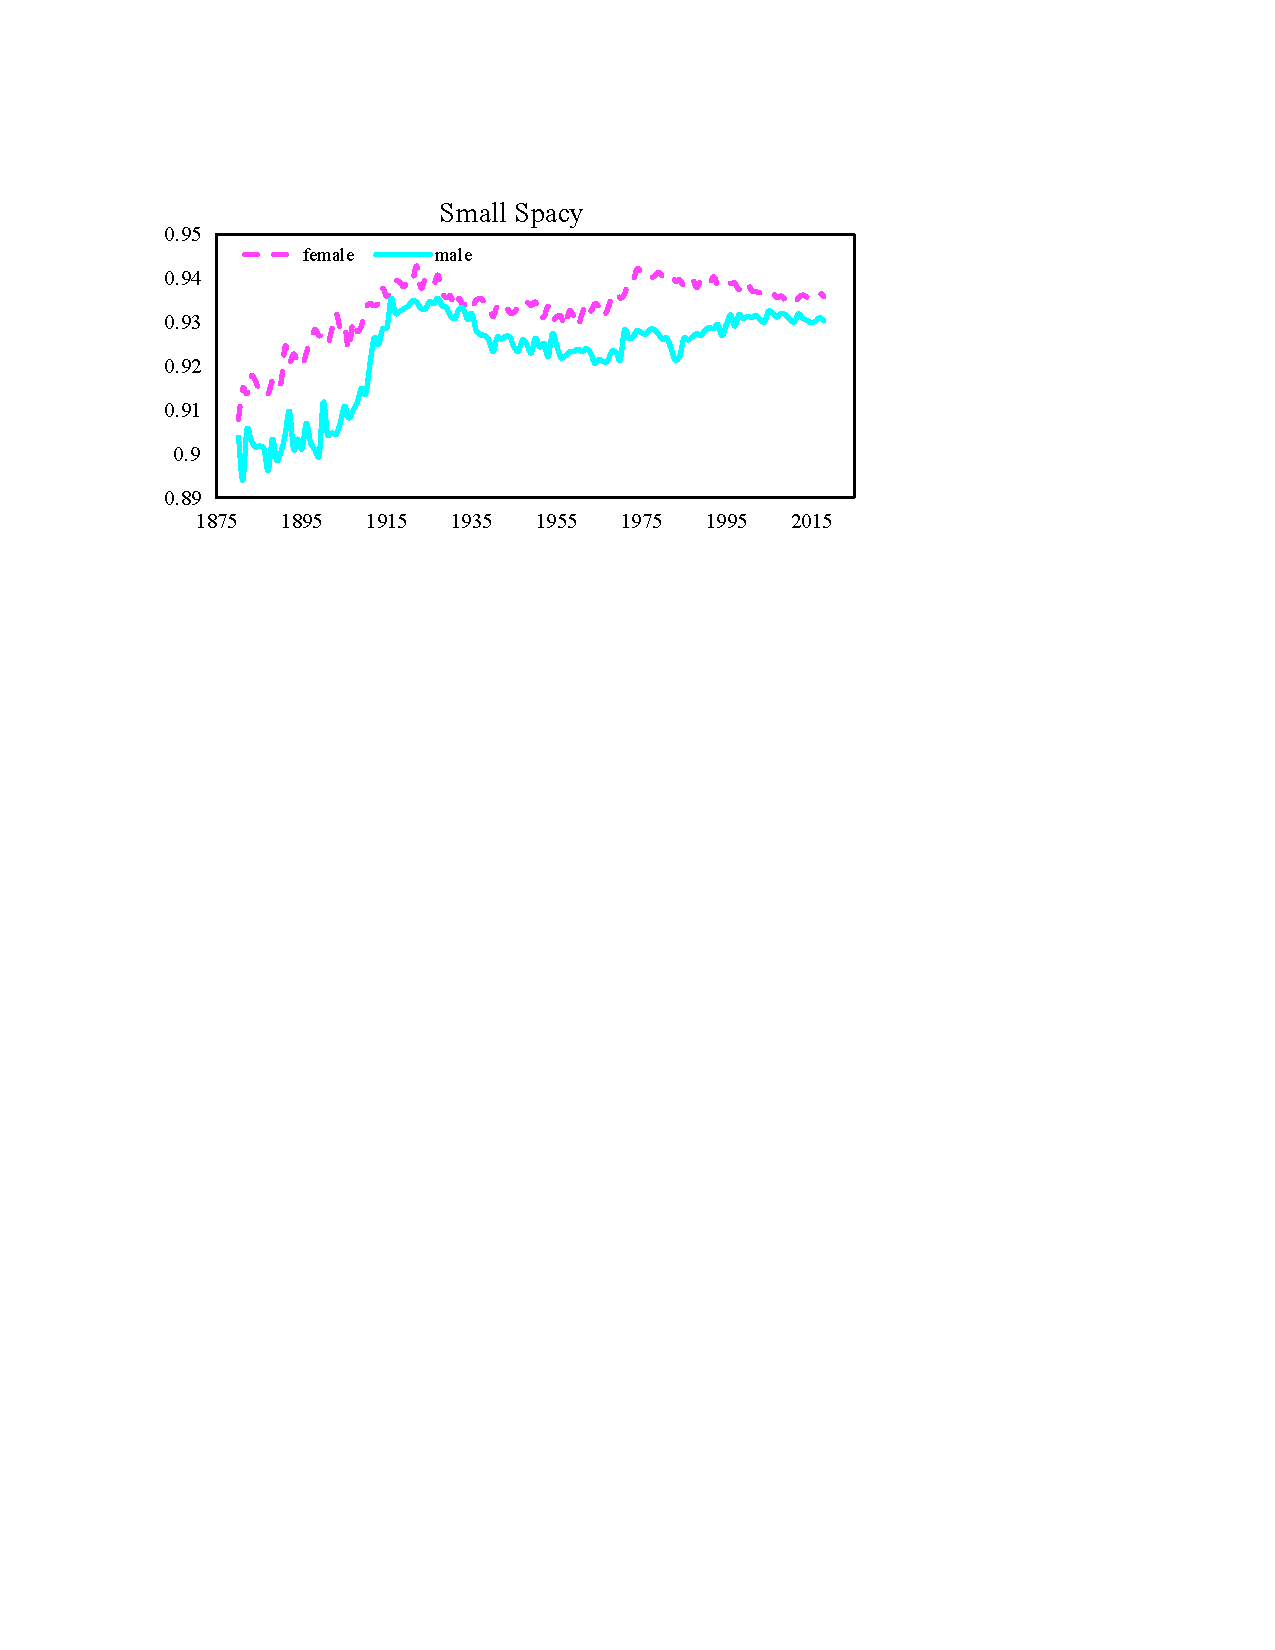
\includegraphics[width=\textwidth,height=0.5\textwidth,trim=0cm 0cm 0cm 0cm,clip=true]{./images/unweighted_type1/unweighted_type1_2.pdf}
\end{subfigure}
\begin{subfigure}[b]{0.33\textwidth}
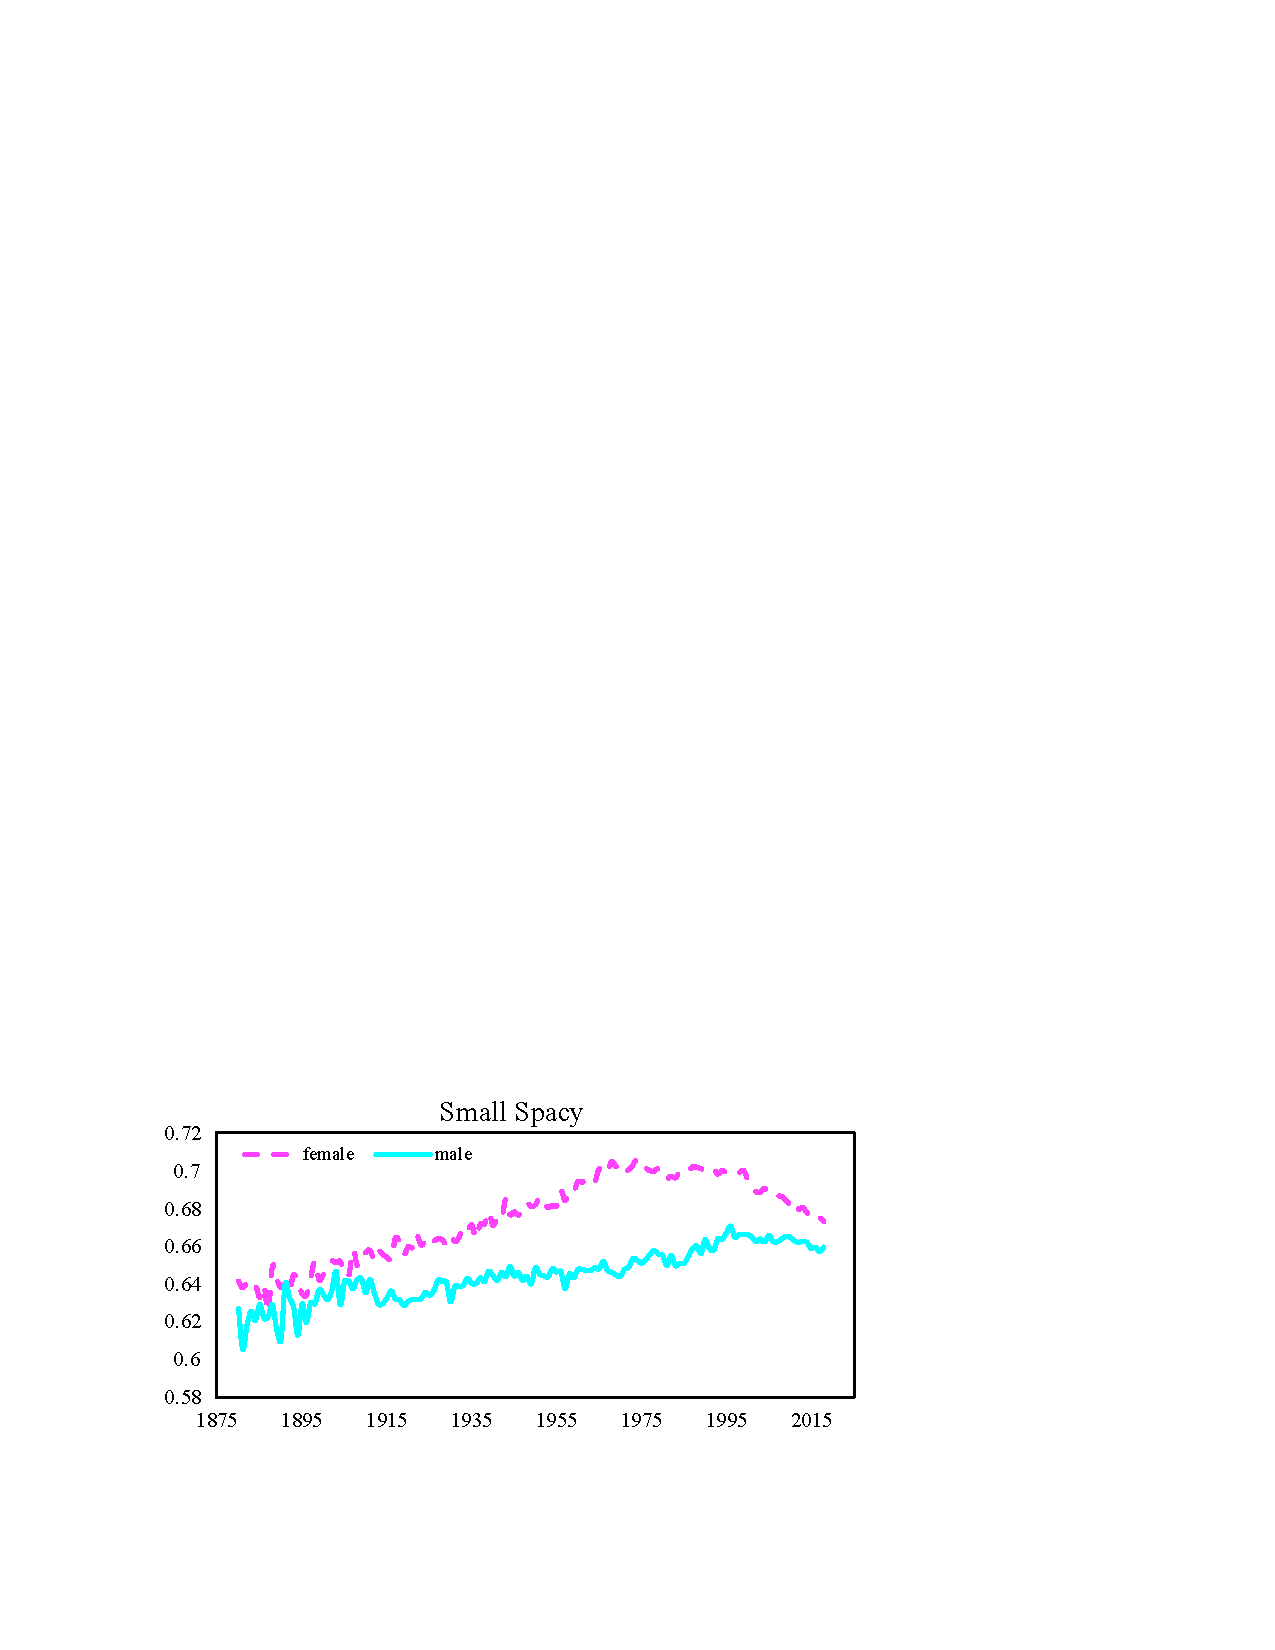
\includegraphics[width=\textwidth,height=0.5\textwidth,trim=0cm 0cm 0cm 0cm,clip=true]{./images/unweighted_type2/unweighted_type2_2.pdf}
\end{subfigure}
\begin{subfigure}[b]{0.33\textwidth}
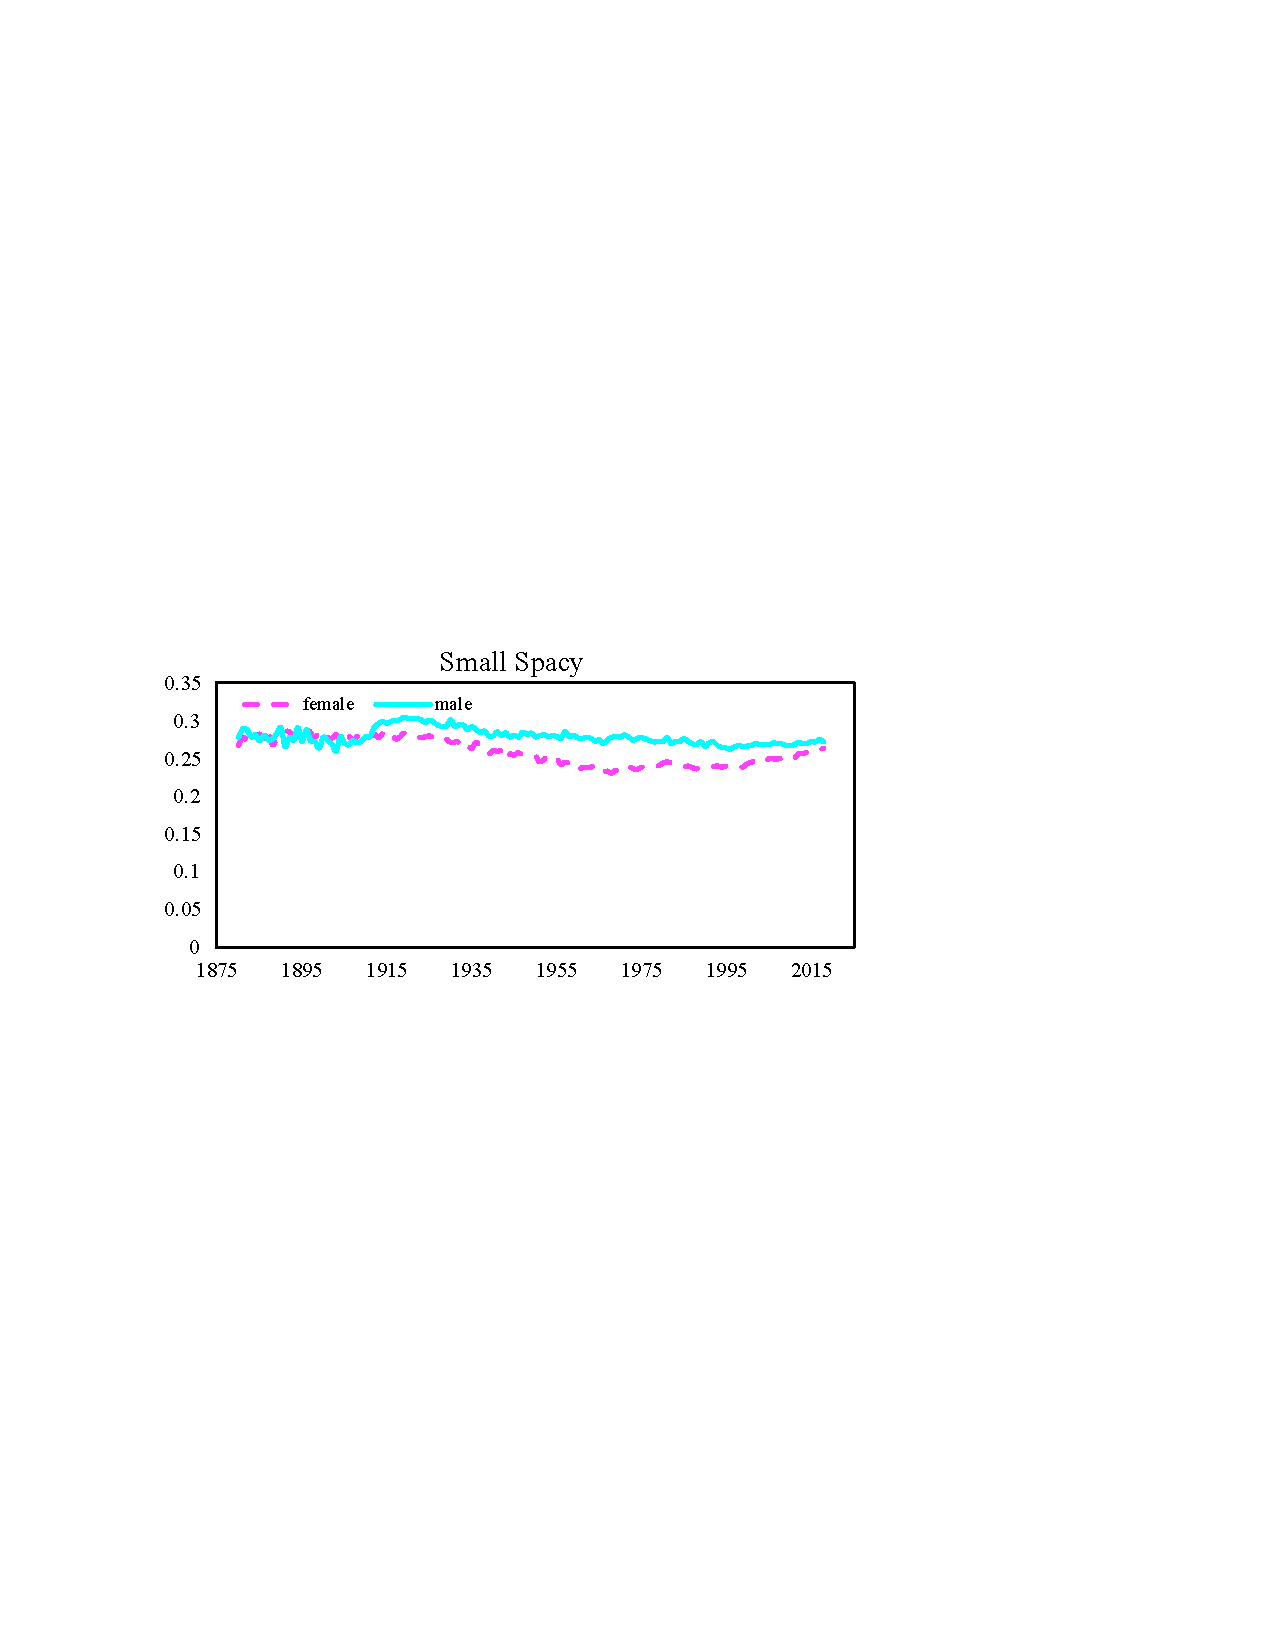
\includegraphics[width=\textwidth,height=0.5\textwidth,trim=0cm 0cm 0cm 0cm,clip=true]{./images/unweighted_type3/unweighted_type3_2.pdf}
\end{subfigure}
\begin{subfigure}[b]{0.33\textwidth}
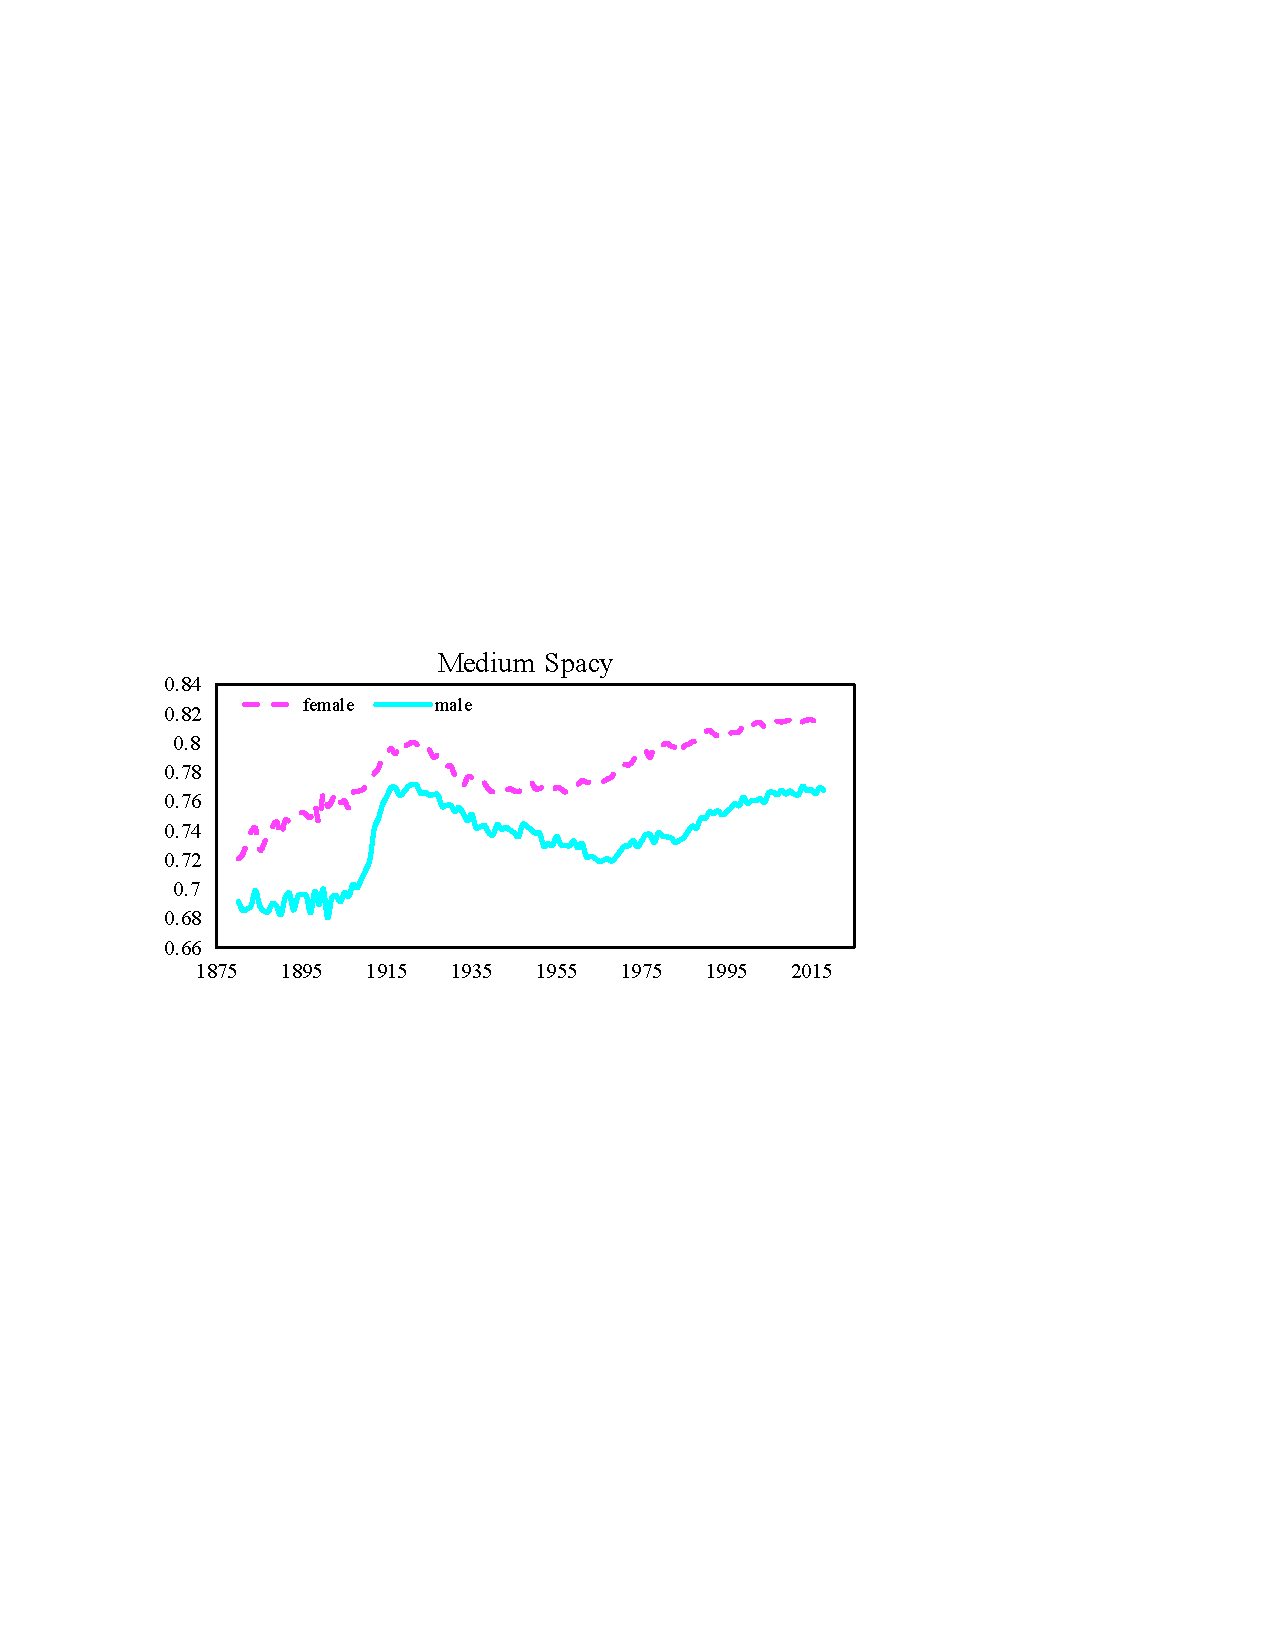
\includegraphics[width=\textwidth,height=0.5\textwidth,trim=0cm 0cm 0cm 0cm,clip=true]{./images/unweighted_type1/unweighted_type1_3.pdf}
\end{subfigure}
\begin{subfigure}[b]{0.33\textwidth}
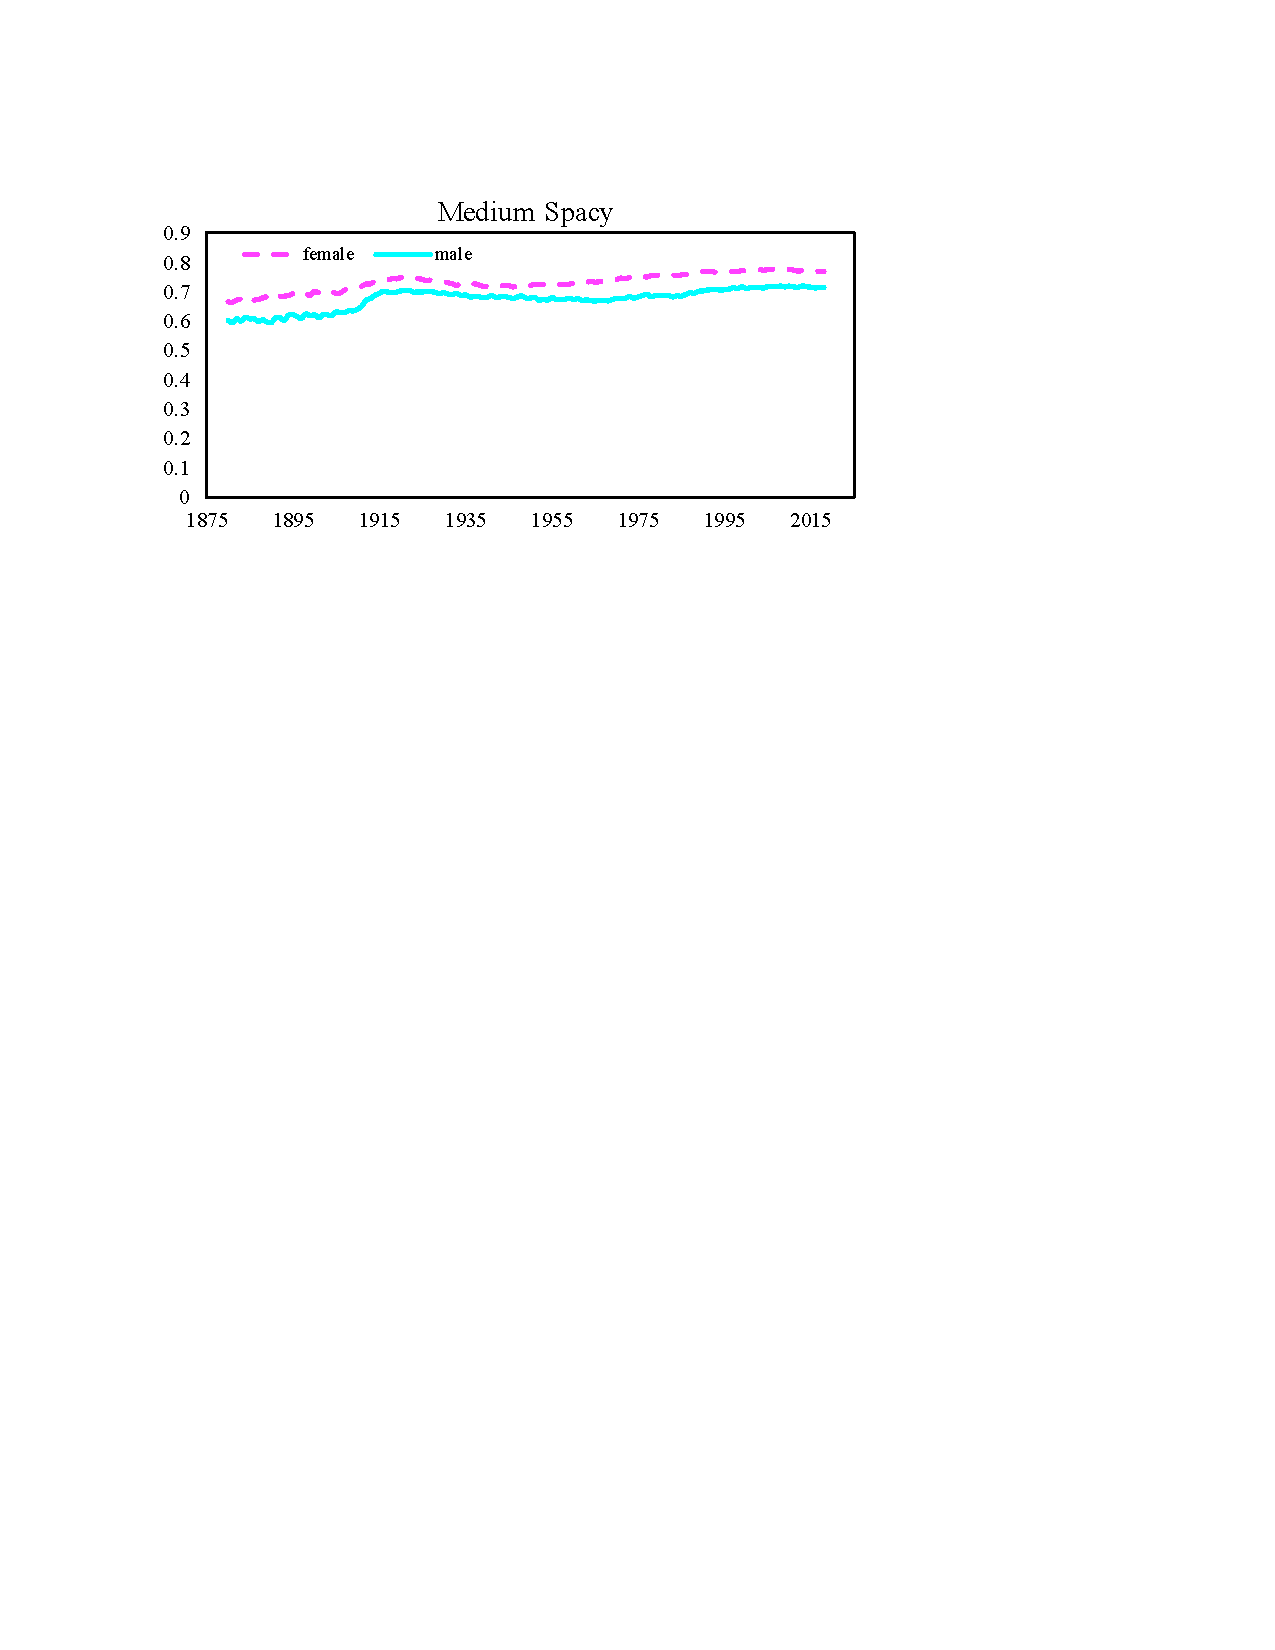
\includegraphics[width=\textwidth,height=0.5\textwidth,trim=0cm 0cm 0cm 0cm,clip=true]{./images/unweighted_type2/unweighted_type2_3.pdf}
\end{subfigure}
\begin{subfigure}[b]{0.33\textwidth}
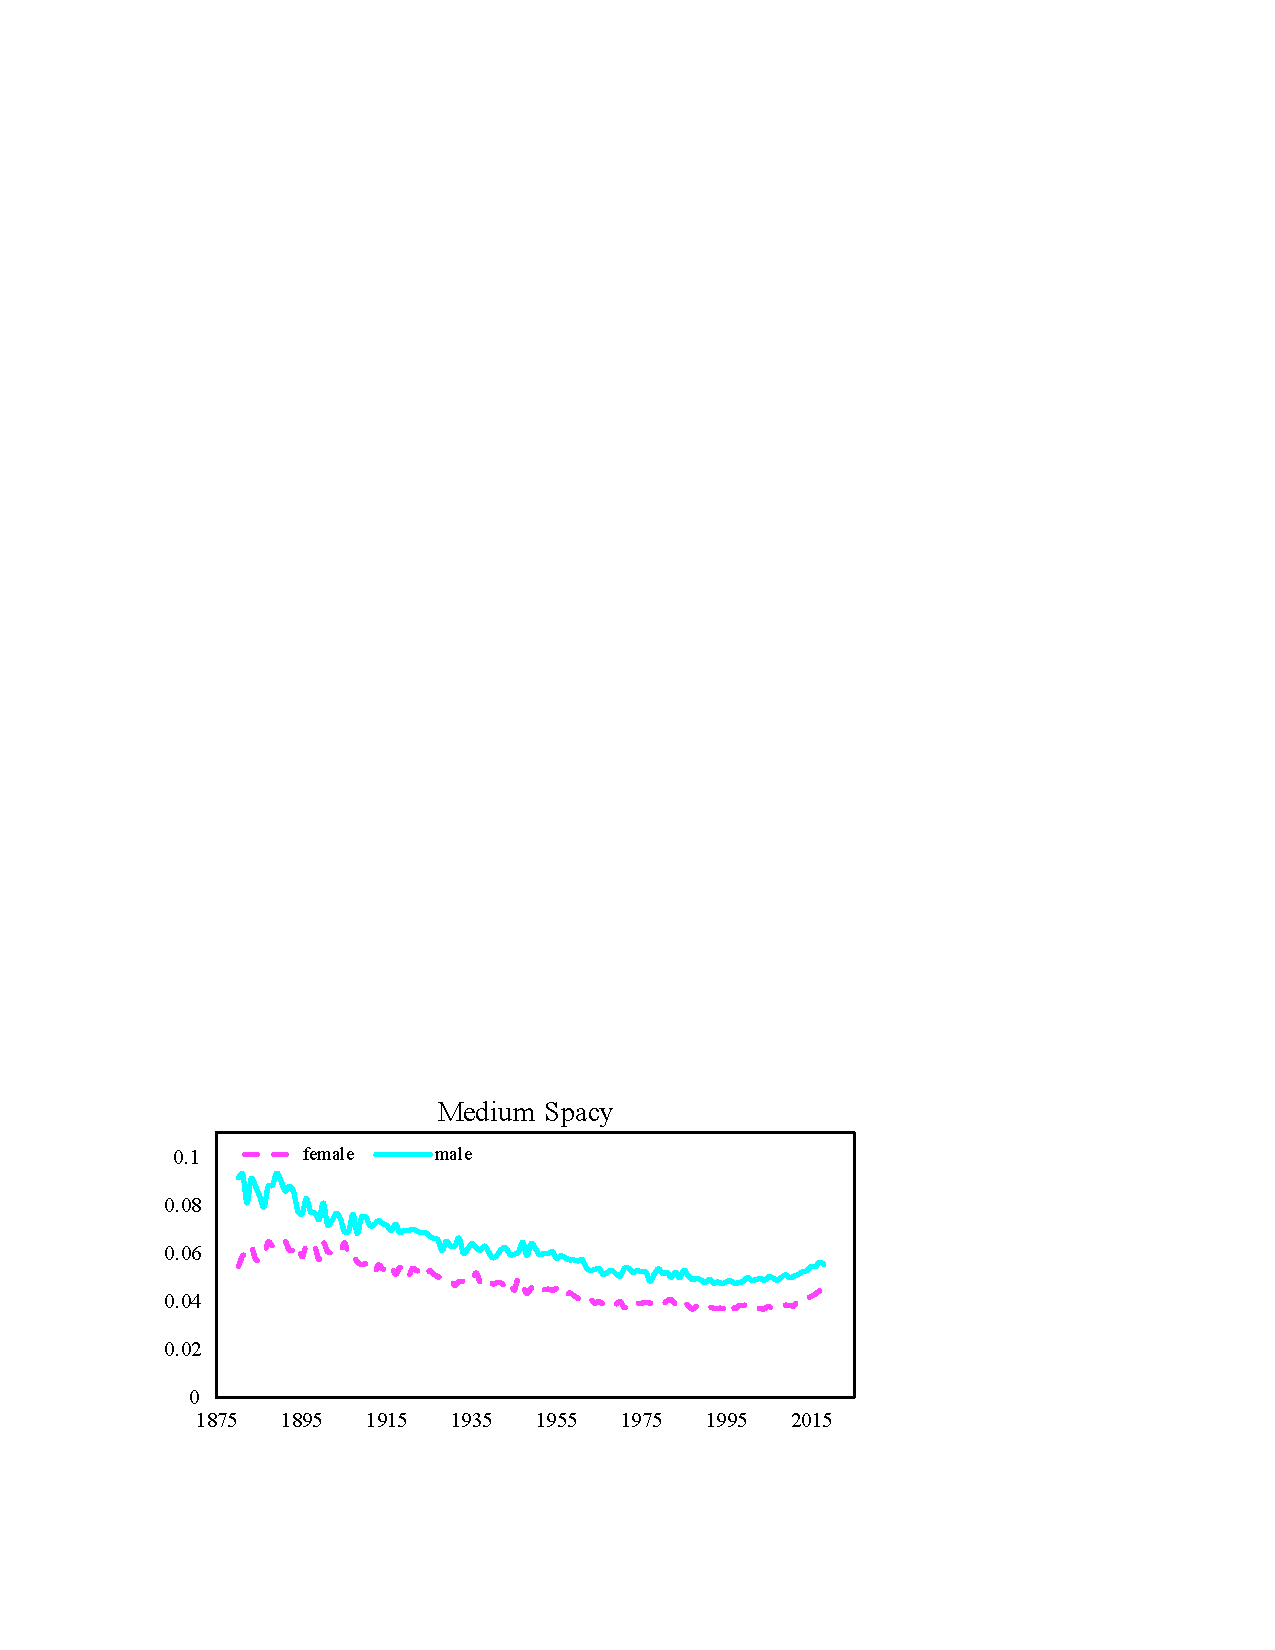
\includegraphics[width=\textwidth,height=0.5\textwidth,trim=0cm 0cm 0cm 0cm,clip=true]{./images/unweighted_type3/unweighted_type3_3.pdf}
\end{subfigure}
\begin{subfigure}[b]{0.33\textwidth}
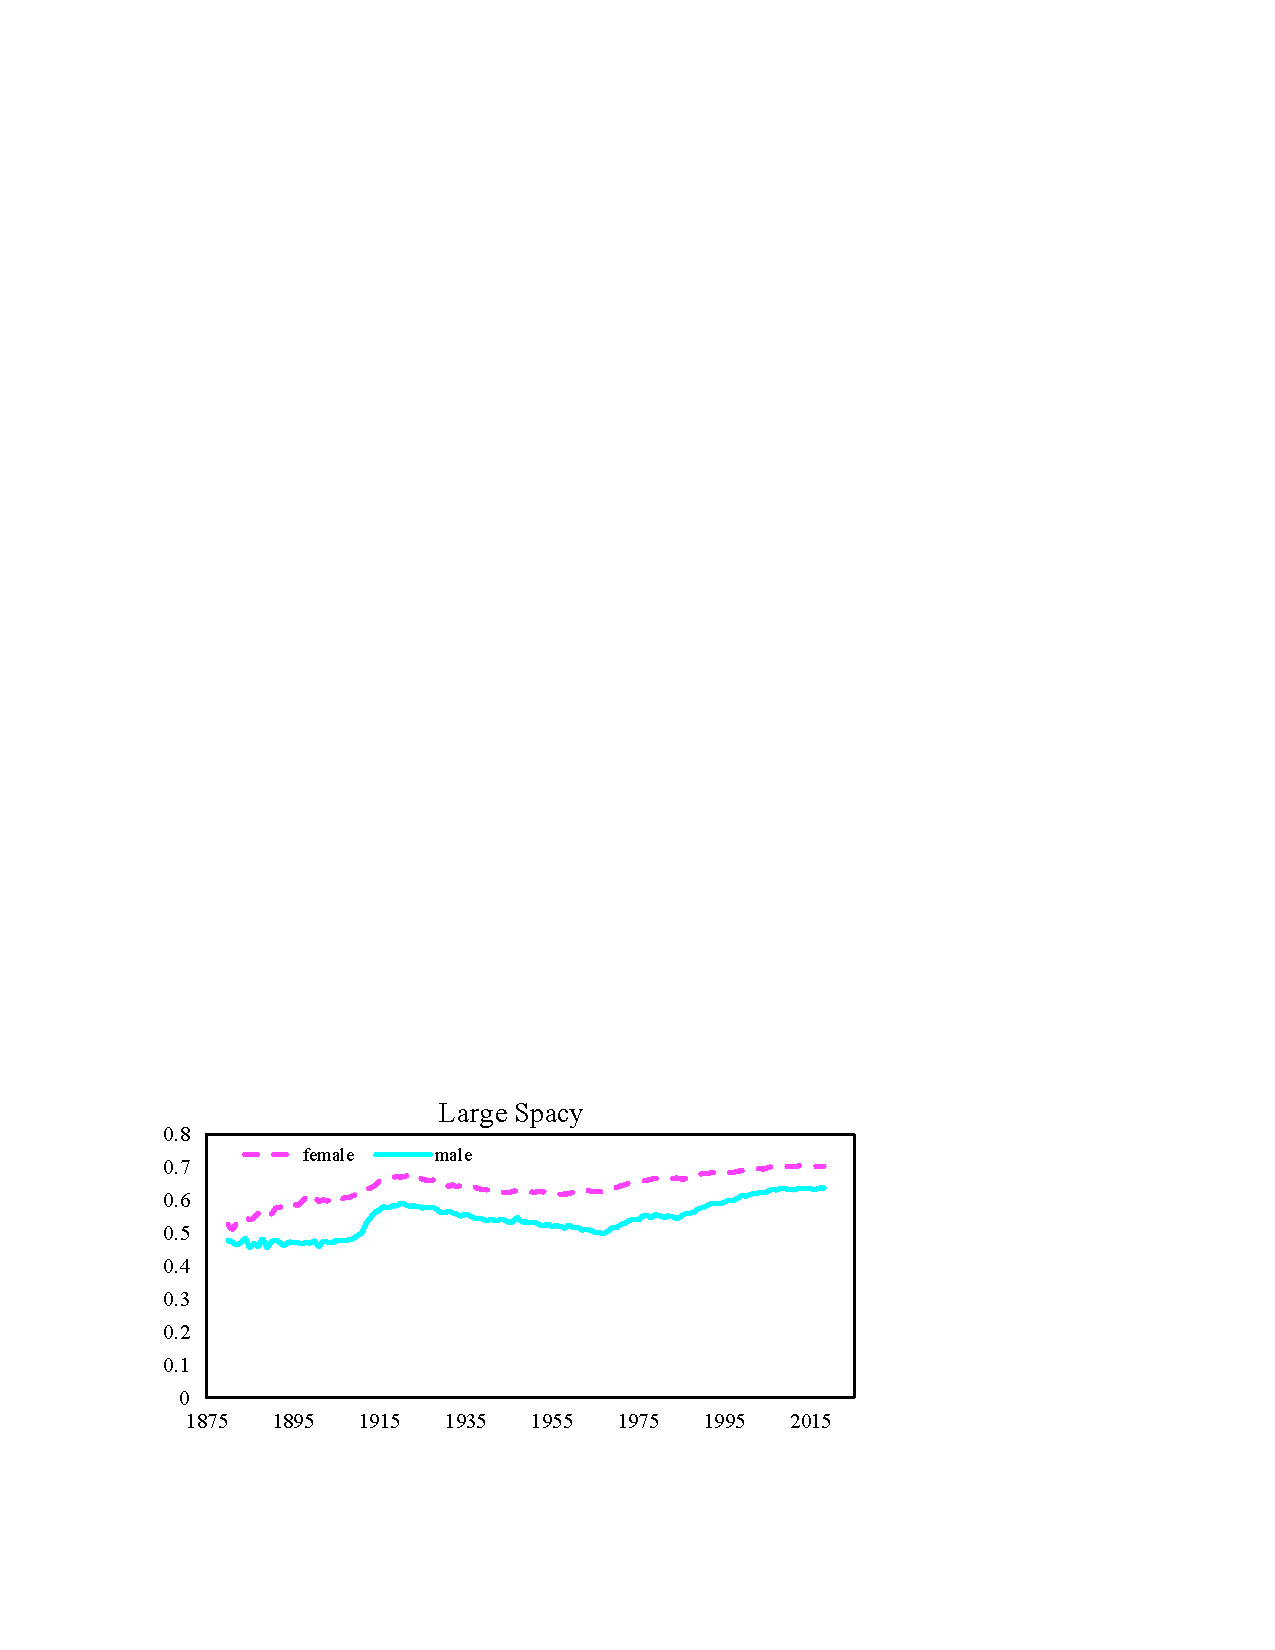
\includegraphics[width=\textwidth,height=0.5\textwidth,trim=0cm 0cm 0cm 0cm,clip=true]{./images/unweighted_type1/unweighted_type1_4.pdf}
\end{subfigure}
\begin{subfigure}[b]{0.33\textwidth}
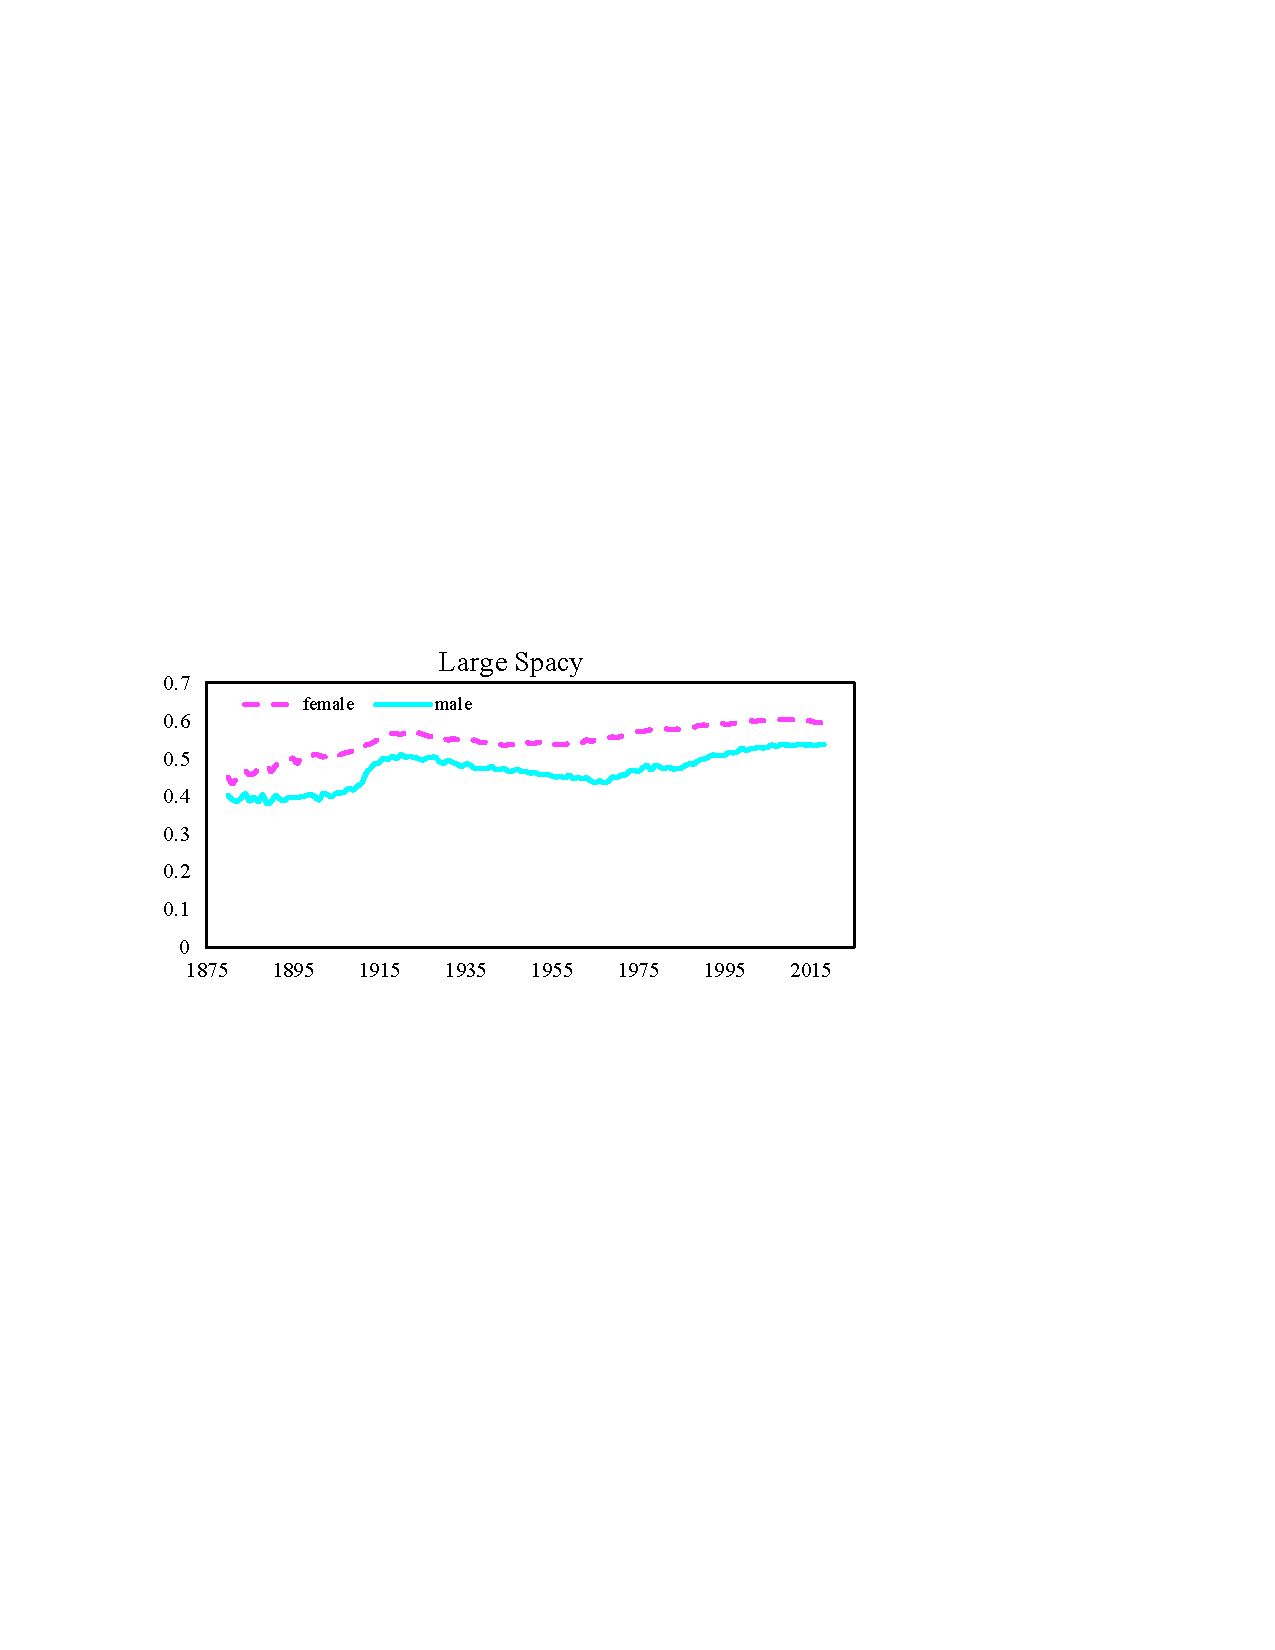
\includegraphics[width=\textwidth,height=0.5\textwidth,trim=0cm 0cm 0cm 0cm,clip=true]{./images/unweighted_type2/unweighted_type2_4.pdf}
\end{subfigure}
\begin{subfigure}[b]{0.33\textwidth}
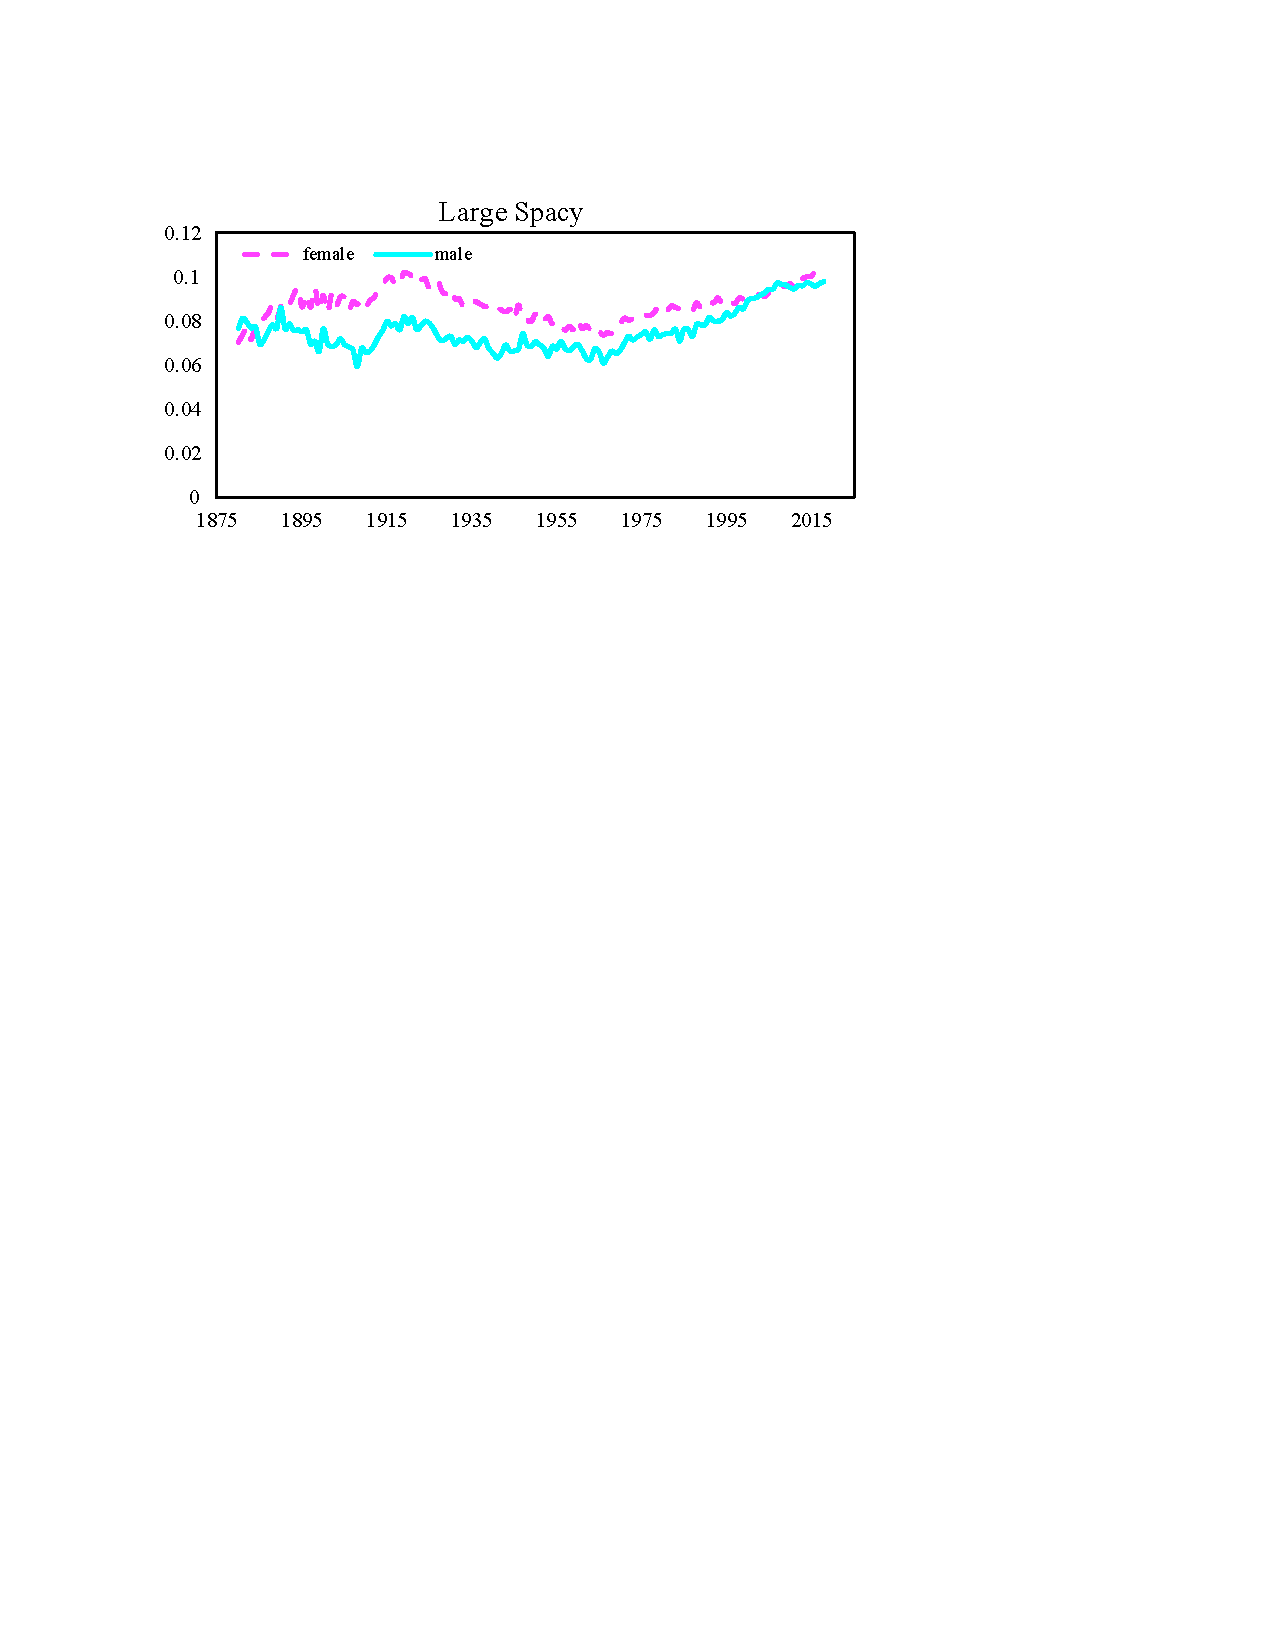
\includegraphics[width=\textwidth,height=0.5\textwidth,trim=0cm 0cm 0cm 0cm,clip=true]{./images/unweighted_type3/unweighted_type3_4.pdf}
\end{subfigure}
\begin{subfigure}[b]{0.33\textwidth}
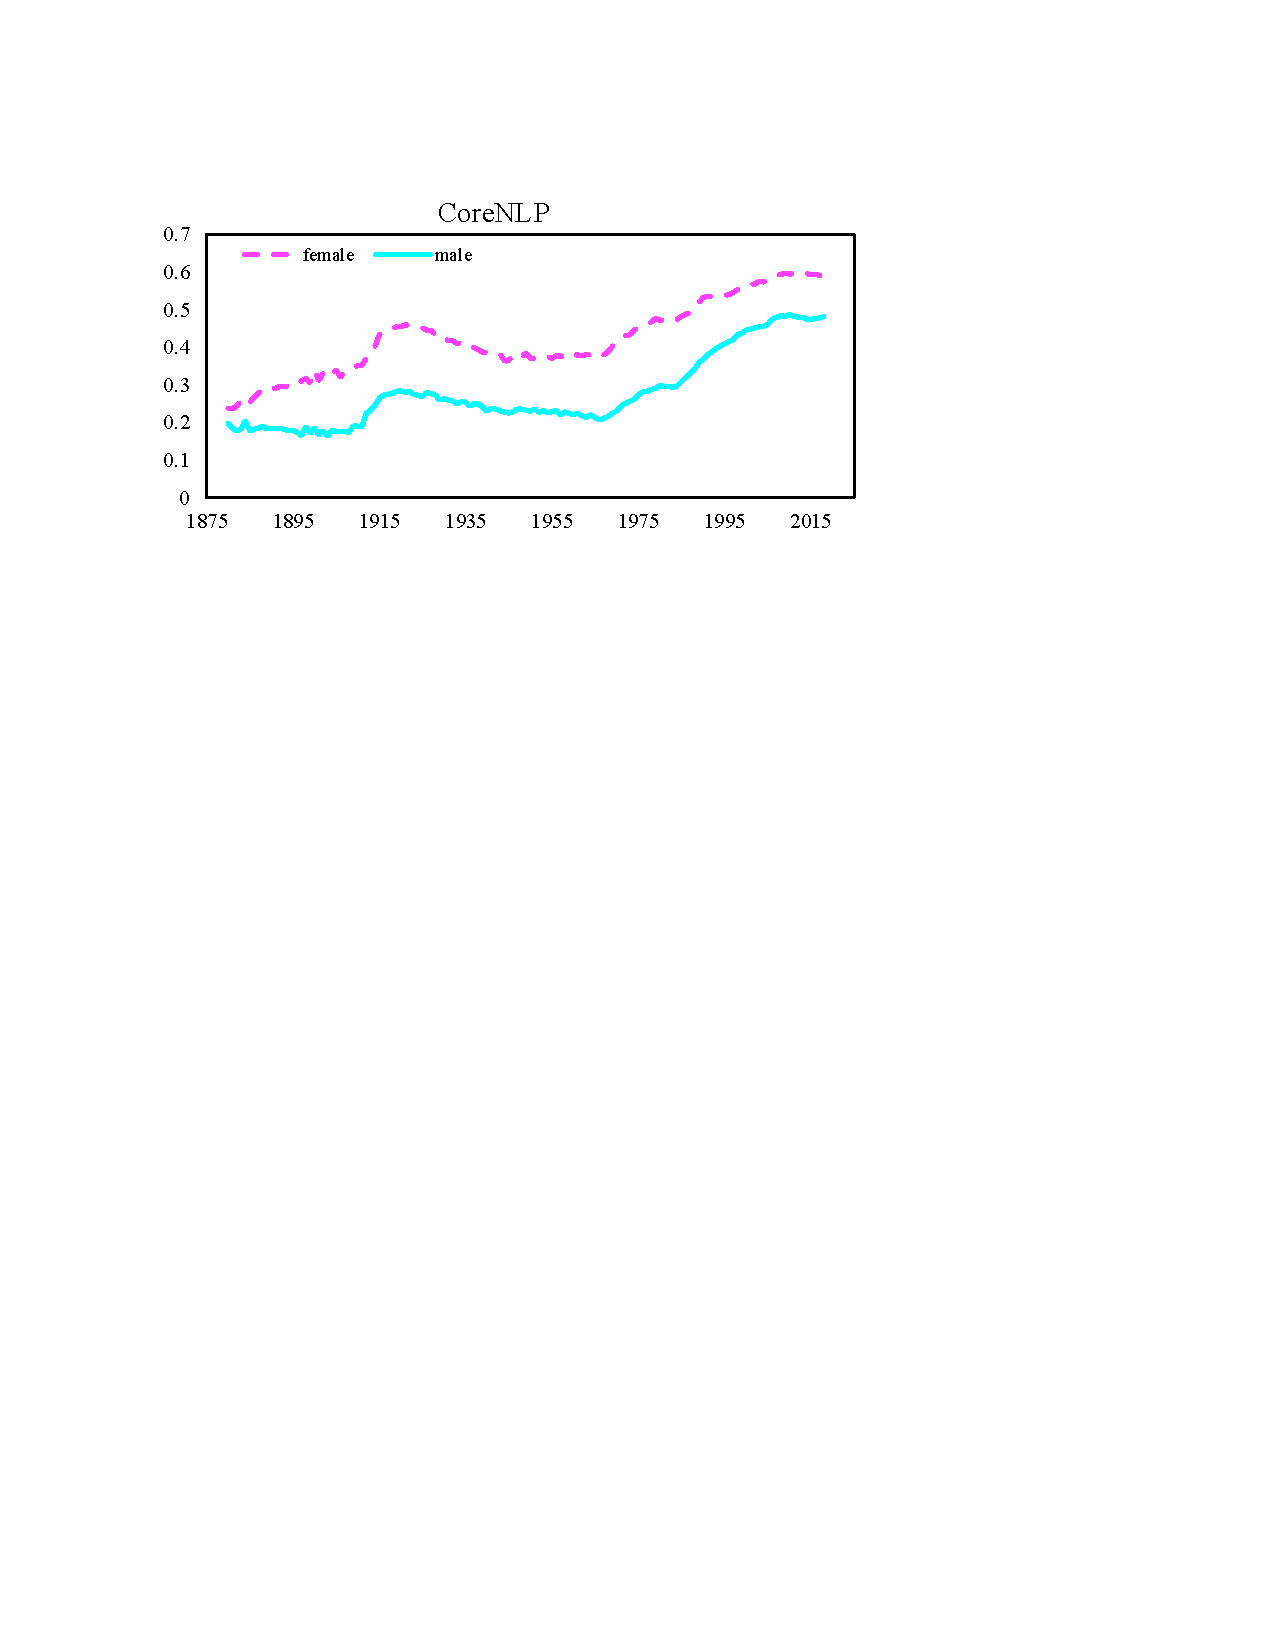
\includegraphics[width=\textwidth,height=0.5\textwidth,trim=0cm 0cm 0cm 0cm,clip=true]{./images/unweighted_type1/unweighted_type1_5.pdf}
\end{subfigure}
\begin{subfigure}[b]{0.33\textwidth}
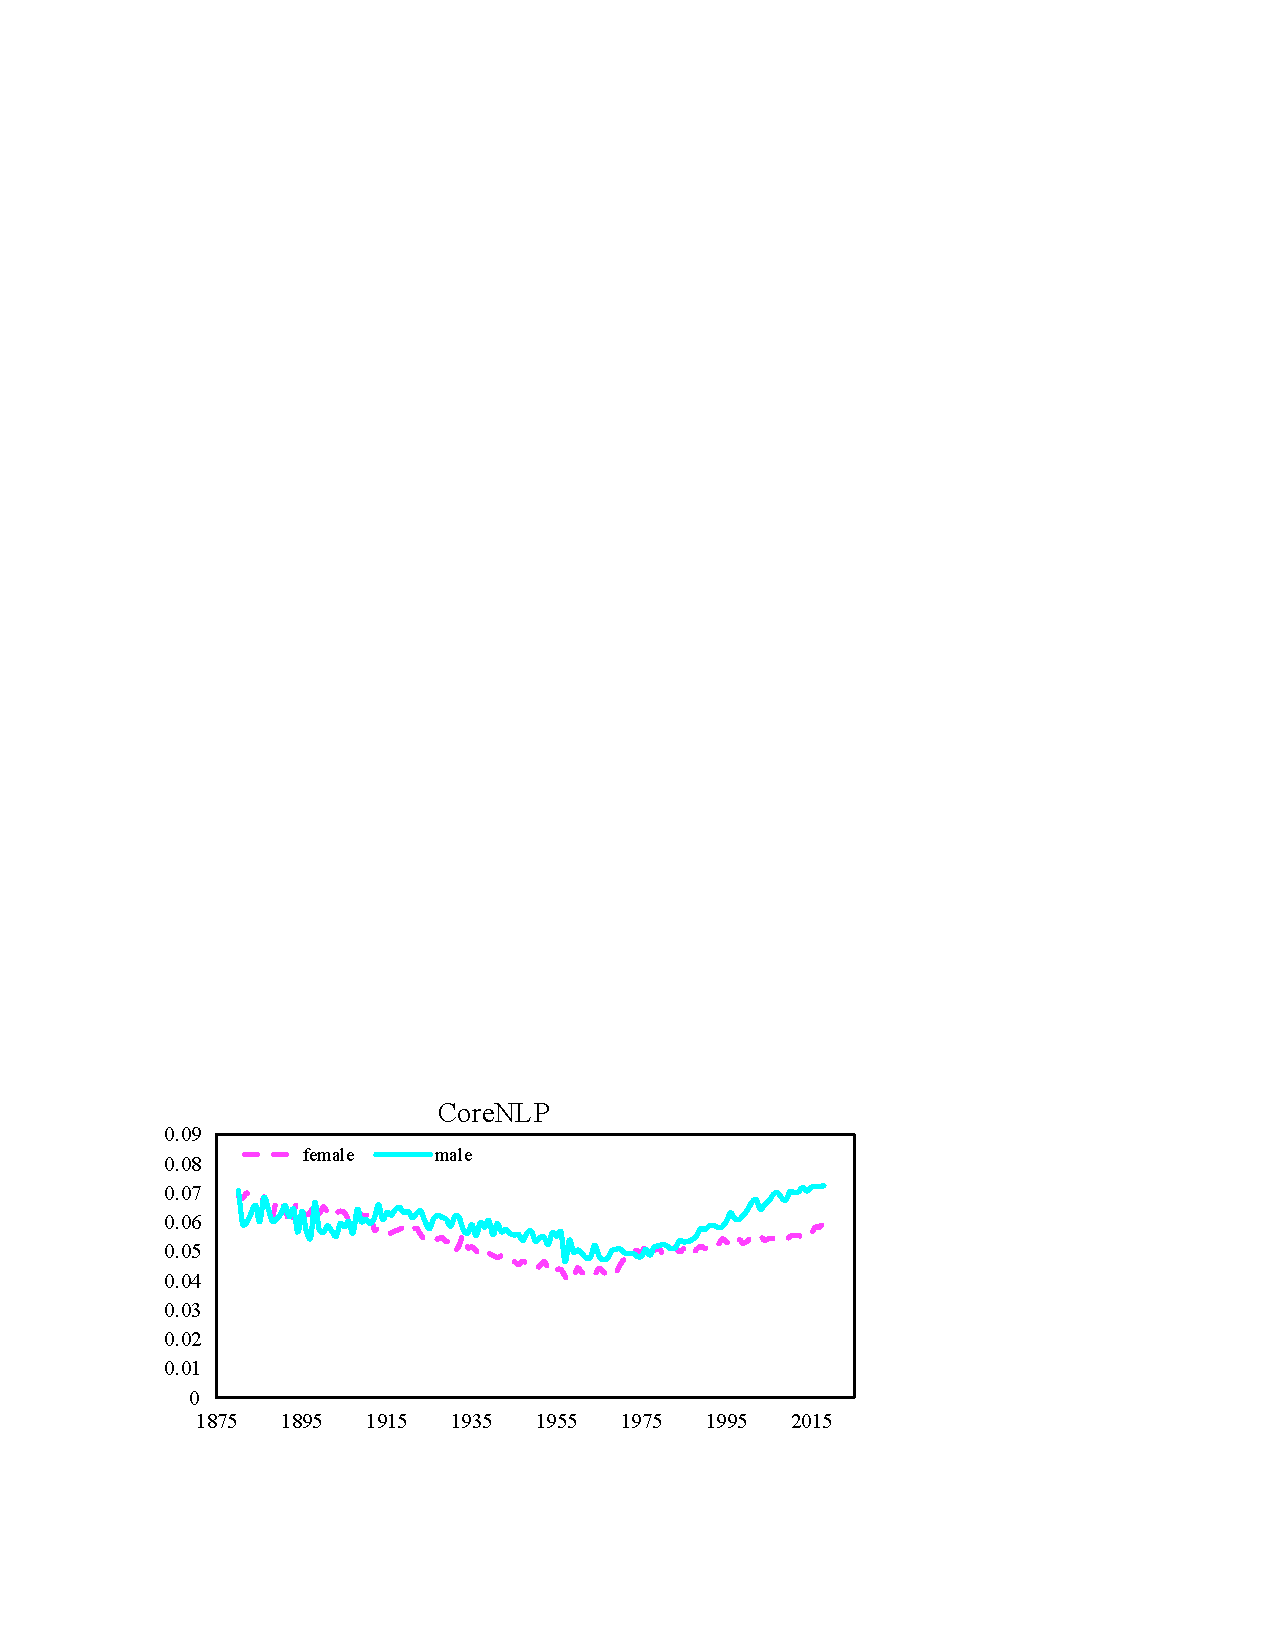
\includegraphics[width=\textwidth,height=0.5\textwidth,trim=0cm 0cm 0cm 0cm,clip=true]{./images/unweighted_type2/unweighted_type2_5.pdf}
\end{subfigure}
\begin{subfigure}[b]{0.33\textwidth}
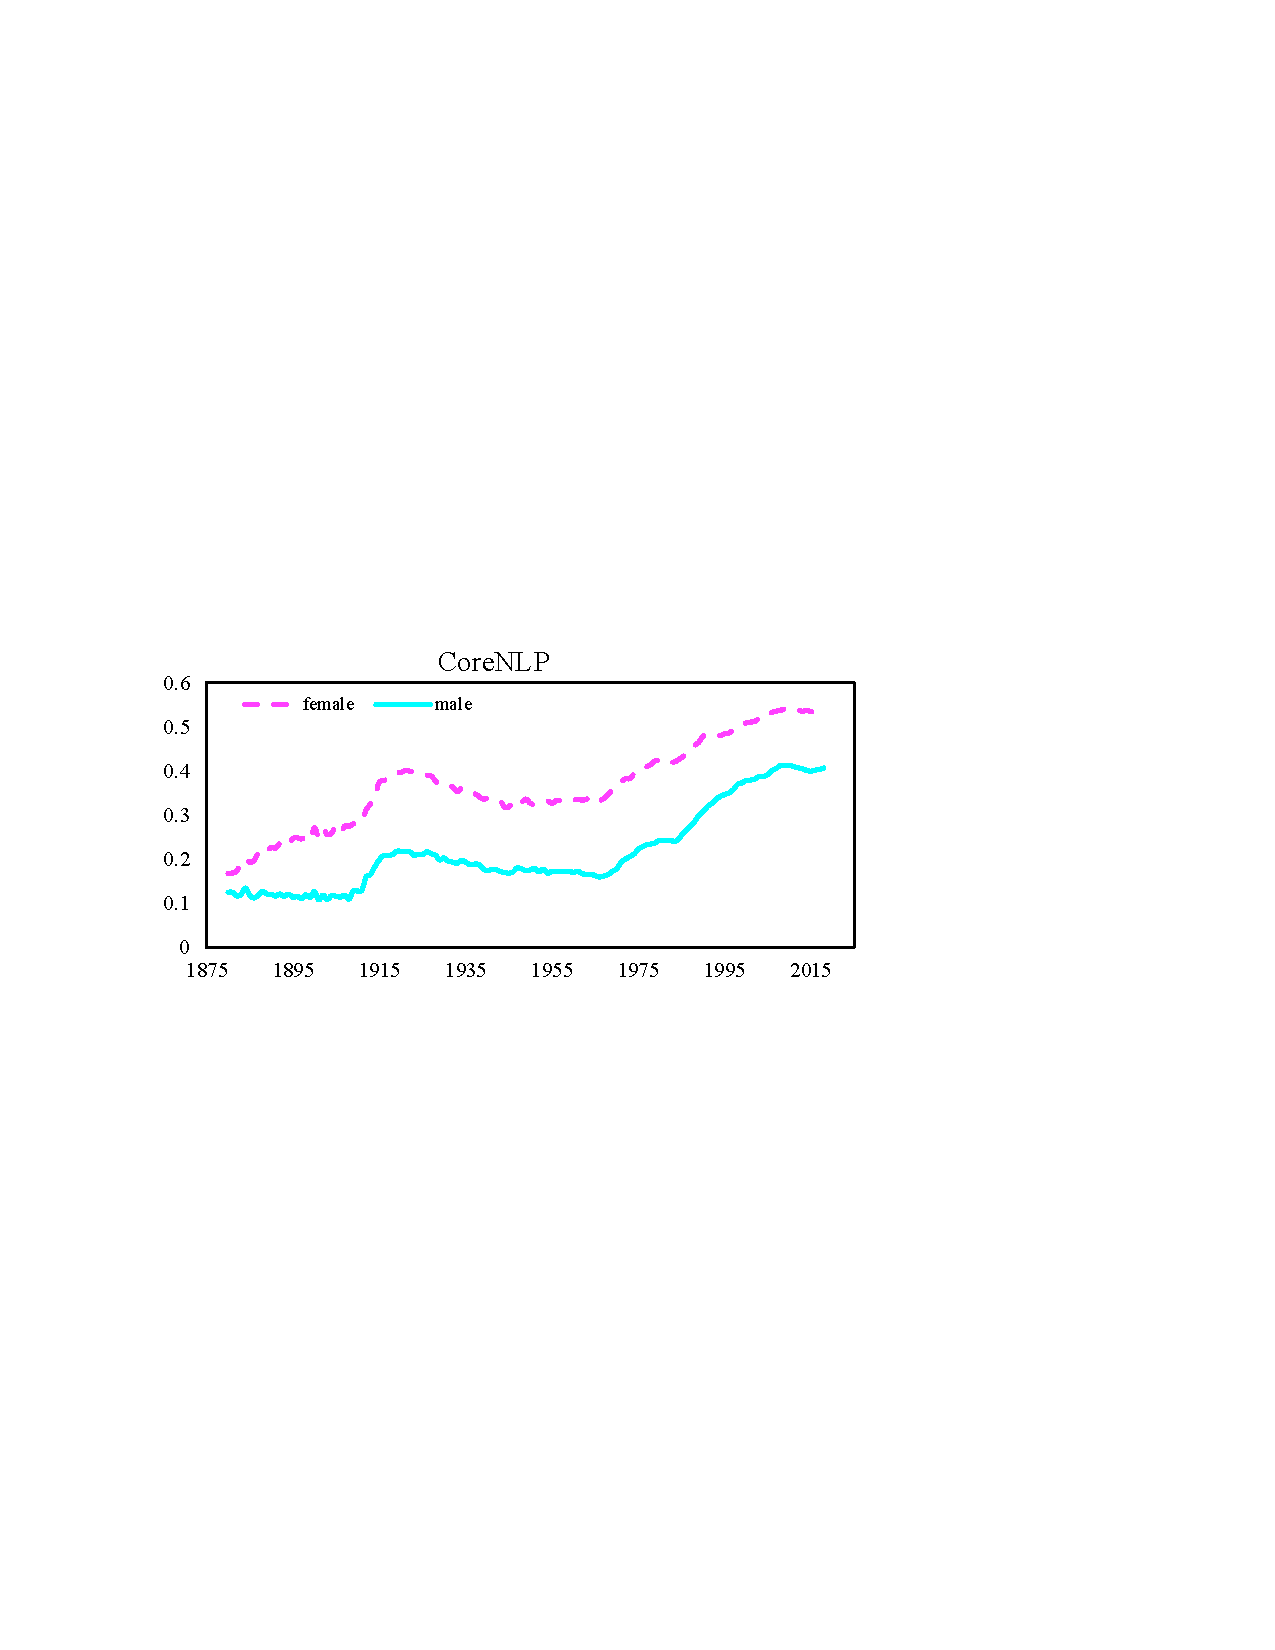
\includegraphics[width=\textwidth,height=0.5\textwidth,trim=0cm 0cm 0cm 0cm,clip=true]{./images/unweighted_type3/unweighted_type3_5.pdf}
\end{subfigure}
\caption{Results from different models over the  139-year history of baby names from the census data on different error types for the unweighted cases using template \#4. Female names have higher error rates for all cases except four marginal cases. The y axis shows the calculated error rates for each of the error types as described in their corresponding formulas, and the x axis represents the year in which the baby name was given.}
\label{result2}
\end{figure*}
Different types of errors allow for fine-grained analysis into the existence of different biases. Our results indicate that all models are mostly more biased toward female names vs. male names, as shown in Figures \ref{result1} and \ref{result2} over the 139-year history. The fact that all the weighted cases are biased toward female names shows that more frequent and popular female names are susceptible to bias and error in named entity recognition systems---which is a more serious type of error to consider. For space considerations, we only report the results for one of the templates (Template \#4) since the results were following similar trend for all the other templates wherein the models were mostly more biased toward female names. We have included results from other templates in our supplementary material to demonstrate that other templates also follow a similar pattern. That being said, in Figure \ref{tempresults} we showed how all the models perform on all the templates, for Error Type-1 Weighted (the super-set error) case, which on its own is showing an interesting trend. This result shows how context helps some models over others by bringing down the error rates when sentences are added to the names (templates \#2 through \#9). Other models perform better on template \#1, showing that context, in fact confuses the model. We observe that in contextual-based models such as Flair, context indeed helps the model make the right decisions by it having less error rates for templates \#2 through \#9 compared to template \#1. Other models do not necessarily follow this pattern. 
As an example, we provide the types of names and errors that can happen in these models. We list the top six most frequent male and female names which were tagged erroneously by the Flair model in year 2018 from our benchmark evaluated on template \#4 in Table \ref{examples}.